\documentclass[10pt]{beamer}

\usetheme{PSY9511}

\usepackage{array}
\usepackage{pgfplots}
\usepackage{tikz}

\title{PSY9511: Seminar 5}
\subtitle{Unsupervised learning}
\author{Esten H. Leonardsen}
\date{24.10.24}

\pgfplotsset{
    discard if not/.style 2 args={
        x filter/.code={
            \edef\tempa{\thisrow{#1}}
            \edef\tempb{#2}
            \ifx\tempa\tempb
            \else
                \def\pgfmathresult{inf}
            \fi
        }
    }
}

\begin{document}
	\begin{frame}
	 	\maketitle
	\end{frame}

    \begin{frame}{Outline}
        \begin{enumerate}
            \item Overview of unsupervised learning
            \item Clustering
            \begin{itemize}
                \item K-means
                \item Hierarchical
            \end{itemize}
            \item Dimensionality reduction
            \begin{itemize}
                \item Principal component analysis (PCA)
                \item Independent component analysis (ICA)
            \end{itemize}
        \end{enumerate}
    \end{frame}

    \section{Unsupervised learning}

\begin{frame}{Unsupervised learning: Motivation}
    \begin{tikzpicture}
        \node[] at (-5.25, 3.5) {};
        \node[] at (-5.25, -3.5) {};

        \node[anchor=north west, font=\bfseries] at (-5, 3) {
            \underline{Supervised learning}: Find $\mathbf{\hat{y}=f(X)}$
        };
        \visible<2-8>{
            \node[anchor=north west, text width=10.5cm, align=left] at (-5, 2.7) {
                \begin{itemize}
                    \item Descriptive: Understand the relationship between $X$ and $y$
                    \item <3-> Predictive: Predict $y$ given new $X$.
                    \begin{itemize}
                        \item <4-> Because the predictions are useful
                        \item <5-> Because we want to know if it is possible
                    \end{itemize}
                \end{itemize}
            };
        }
        \visible<2>{
            \node[] at (0, -1) {
                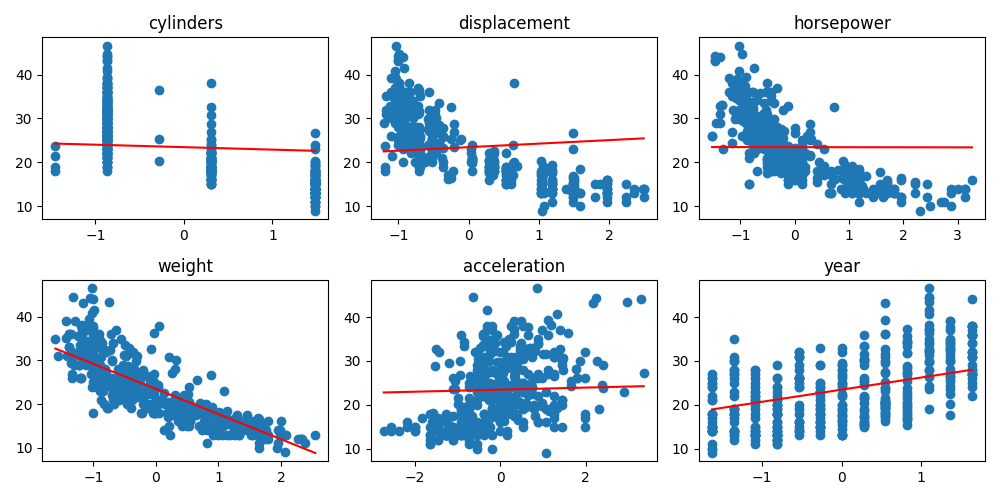
\includegraphics[height=4cm]{data/coefficients.png}
            };
        }
        \visible<4>{
            \node[] at (0, -1.5) {
                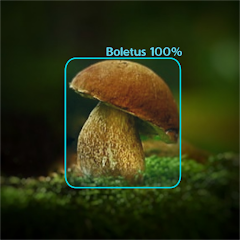
\includegraphics[height=3cm]{data/mushroom.png}
            };
        }
        \visible<5>{
            \node[] (mri) at (-2, -1.5) {
                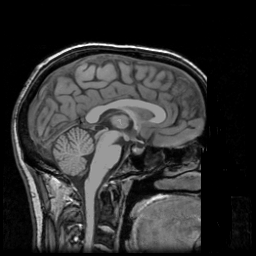
\includegraphics[height=2.5cm]{data/brain.png}
            };
            \node[draw=black, dashed] (outcome) at (2, -1.5) {
                Depression?
            };
            \draw[-stealth, line width=5pt, gray] (mri) -- (outcome);
        }
        \visible<6-8>{
            \node[anchor=north west, font=\bfseries] at (-5, 0) {
                \underline{Unsupervised learning}: Are there some interesting patterns in $\mathbf{X}$?
            };
        }
        \visible<7-8>{
            \node[anchor=north west, text width=10.5cm, align=left] at (-5, -0.3) {
                \begin{itemize}
                    \item Can we find subgroups or interesting axes of variability?
                    \item <8> Exploratory analyses
                    \item <8> Visualization
                \end{itemize}
            };
        }
    \end{tikzpicture}
\end{frame}

    \section{Clustering}

\newcommand{\clusterplot}[1]{
    \begin{tikzpicture}
        \begin{axis}[
            height=6cm,
            width=6cm,
            xmajorticks=false,
            ymajorticks=false,
            xlabel=$x_1$,
            ylabel=$x_2$,
        ]
            \ifnum#1=0
                \addplot[
                    only marks,
                    mark=*,
                    blue,
                    opacity=0.5
                ] table [
                    col sep=comma,
                    x=x,
                    y=y
                ]{data/clusterdata.csv};
            \fi
            \ifnum#1=1
                \addplot[
                    only marks,
                    mark=*,
                    blue,
                    opacity=0.5
                ] table [
                    col sep=comma,
                    x=x,
                    y=y,
                    discard if not={c}{0.0}
                ]{data/clusterdata.csv};

                \addplot[
                    only marks,
                    mark=*,
                    green,
                    opacity=0.5
                ] table [
                    col sep=comma,
                    x=x,
                    y=y,
                    discard if not={c}{1.0}
                ]{data/clusterdata.csv};

                \addplot[
                    only marks,
                    mark=*,
                    red,
                    opacity=0.5
                ] table [
                    col sep=comma,
                    x=x,
                    y=y,
                    discard if not={c}{2.0}
                ]{data/clusterdata.csv};
            \fi
        \end{axis}
    \end{tikzpicture}
}

\newsavebox{\unclusteredbox}
\sbox{\unclusteredbox}{
    \clusterplot{0}
}
\newsavebox{\clusteredbox}
\sbox{\clusteredbox}{
    \clusterplot{1}
}

\begin{frame}{Clustering: Background}
    \begin{tikzpicture}
        \node[] at (-5.25, 3.5) {};
        \node[] at (-5.25, -3.5) {};

        \visible<1-4>{
            \node[] at (0, 3) {
                Are there some (naturally occuring) subgroups in our dataset?
            };
        }
        \visible<2-5>{
            \node[anchor=north west] at (-4.5, 2.5) {
                \begin{tabular}{|>{\centering\arraybackslash}p{1cm}|>{\centering\arraybackslash}p{1cm}|}
                    \hline
                    $\mathbf{x_1}$ & $\mathbf{x_2}$ \\
                    \hline
                    0.20&-0.26\\
                    0.15&-0.33\\
                    0.03&0.07\\
                    -0.07&-0.01\\
                    -0.06&0.00\\
                    0.28&-0.24\\
                    0.21&-0.35\\
                    0.20&-0.32\\
                    0.30&0.25\\
                    0.00&-0.12\\
                    \hline
                \end{tabular}
            };
        }
        \visible<3>{
            \node[anchor=north east] at (4.5, 2) {
                \usebox{\unclusteredbox}
            };
        }
        \visible<4-5>{
            \node[anchor=north east] at (4.5, 2) {
                \usebox{\clusteredbox}
            };
        }
        \visible<5>{
            \node[] at (0, 3) {
                Are there some (\textcolor{red}{naturally occuring}) subgroups in our dataset?
            };
        }
    \end{tikzpicture}
\end{frame}

\newcommand{\simpleclusterplot}[1]{
    \begin{tikzpicture}
        \begin{axis}[
            height=5.45cm,
            width=5.45cm,
            xmajorticks=false,
            ymajorticks=false,
            xlabel=$x_1$,
            ylabel=$x_2$
        ]
            \ifnum#1=0
                \addplot[
                    only marks,
                    blue,
                    opacity=0.5
                ] coordinates {
                    (1, 1)
                    (1.5, 1)
                    (1.25, 1.25)
                    (-1, 1)
                    (-1.5, 1)
                    (-1.25, 1.25)
                    (0.25, 0.0)
                    (-0.25, 0.0)
                    (0, -0.25)
                };
            \fi
            \ifnum#1=1
                \addplot[
                    only marks,
                    blue,
                    opacity=0.5
                ] coordinates {
                    (1, 1)
                    (1.5, 1)
                    (1.25, 1.25)
                };
                \addplot[
                    only marks,
                    green,
                    opacity=0.5
                ] coordinates {
                    (-1, 1)
                    (-1.5, 1)
                    (-1.25, 1.25)
                };
                \addplot[
                    only marks,
                    red,
                    opacity=0.5
                ] coordinates {
                    (0.25, 0.0)
                    (-0.25, 0.0)
                    (0, -0.25)
                };
            \fi
            \ifnum#1=2
                \addplot[
                    only marks,
                    blue,
                    opacity=0.5
                ] coordinates {
                    (1, 1)
                    (-1, 1)
                    (0.25, 0.0)
                };
                \addplot[
                    only marks,
                    green,
                    opacity=0.5
                ] coordinates {
                    (-1.5, 1)
                    (1.5, 1)
                    (-0.25, 0.0)
                };
                \addplot[
                    only marks,
                    red,
                    opacity=0.5
                ] coordinates {
                    (0, -0.25)
                    (-1.25, 1.25)
                    (1.25, 1.25)
                };
            \fi
            \ifnum#1=3
                \addplot[
                    only marks,
                    blue,
                    opacity=0.5
                ] coordinates {
                    (1, 1)
                    (1.5, 1)
                    (1.25, 1.25)
                };
                \addplot[
                    only marks,
                    green!25,
                    opacity=0.5
                ] coordinates {
                    (-1, 1)
                    (-1.5, 1)
                    (-1.25, 1.25)
                };
                \addplot[
                    only marks,
                    red!25,
                    opacity=0.5
                ] coordinates {
                    (0.25, 0.0)
                    (-0.25, 0.0)
                    (0, -0.25)
                };
            \fi
            \ifnum#1=4
                \addplot[
                    only marks,
                    blue,
                    opacity=0.5
                ] coordinates {
                    (1, 1)
                    (1.5, 1)
                };
                \addplot[
                    only marks,
                    blue!25,
                    opacity=0.5
                ] coordinates {
                    (1.25, 1.25)
                };
                \addplot[
                    only marks,
                    green!25,
                    opacity=0.5
                ] coordinates {
                    (-1, 1)
                    (-1.5, 1)
                    (-1.25, 1.25)
                };
                \addplot[
                    only marks,
                    red!25,
                    opacity=0.5
                ] coordinates {
                    (0.25, 0.0)
                    (-0.25, 0.0)
                    (0, -0.25)
                };
            \fi
            \ifnum#1=5
                \addplot[
                    only marks,
                    blue,
                    opacity=0.5
                ] coordinates {
                    (1, 1)
                    (1.25, 1.25)
                };
                \addplot[
                    only marks,
                    blue!25,
                    opacity=0.5
                ] coordinates {
                    (1.5, 1)
                };
                \addplot[
                    only marks,
                    green!25,
                    opacity=0.5
                ] coordinates {
                    (-1, 1)
                    (-1.5, 1)
                    (-1.25, 1.25)
                };
                \addplot[
                    only marks,
                    red!25,
                    opacity=0.5
                ] coordinates {
                    (0.25, 0.0)
                    (-0.25, 0.0)
                    (0, -0.25)
                };
            \fi
            \ifnum#1>5
                \addplot[
                    only marks,
                    blue,
                    opacity=0.5
                ] coordinates {
                    (1.25, 1.25)
                    (1.5, 1)
                };
                \addplot[
                    only marks,
                    blue!25,
                    opacity=0.5
                ] coordinates {
                    (1, 1)
                };
                \addplot[
                    only marks,
                    green!25,
                    opacity=0.5
                ] coordinates {
                    (-1, 1)
                    (-1.5, 1)
                    (-1.25, 1.25)
                };
                \addplot[
                    only marks,
                    red!25,
                    opacity=0.5
                ] coordinates {
                    (0.25, 0.0)
                    (-0.25, 0.0)
                    (0, -0.25)
                };
            \fi
            \ifnum#1>6
                \draw[] (axis cs: 1.25, 1.25) -- (axis cs: 1.5, 1.25);
            \fi
            \ifnum#1>7
                \draw[] (axis cs: 1.5, 1.25) -- (axis cs: 1.5, 1);
            \fi
            \ifnum#1>8
                \draw[red,stealth-stealth] (axis cs: 1.25, 1.25) -- (axis cs: 1.5, 1);
            \fi
        \end{axis}
    \end{tikzpicture}
}

\newsavebox{\simpleunclustered}
\sbox{\simpleunclustered}{
    \simpleclusterplot{0}
}
\newsavebox{\simpleclustered}
\sbox{\simpleclustered}{
    \simpleclusterplot{1}
}
\newsavebox{\simplebad}
\sbox{\simplebad}{
    \simpleclusterplot{2}
}
\newsavebox{\simplesingle}
\sbox{\simplesingle}{
    \simpleclusterplot{3}
}
\newsavebox{\simplefirst}
\sbox{\simplefirst}{
    \simpleclusterplot{4}
}
\newsavebox{\simplesecond}
\sbox{\simplesecond}{
    \simpleclusterplot{5}
}
\newsavebox{\simplethird}
\sbox{\simplethird}{
    \simpleclusterplot{6}
}
\newsavebox{\firstdistance}
\sbox{\firstdistance}{
    \simpleclusterplot{7}
}
\newsavebox{\seconddistance}
\sbox{\seconddistance}{
    \simpleclusterplot{8}
}
\newsavebox{\thirddistance}
\sbox{\thirddistance}{
    \simpleclusterplot{9}
}

\newsavebox{\exponential}
\sbox{\exponential}{
    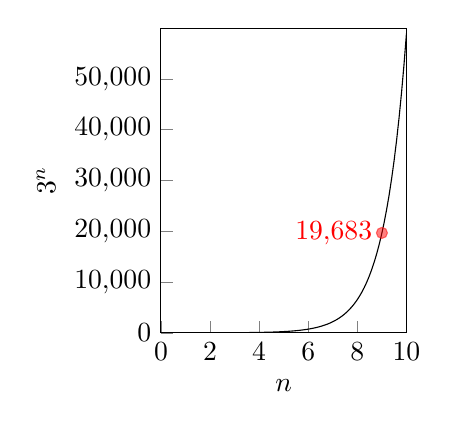
\begin{tikzpicture}
        \begin{axis}[
            height=5.45cm,
            width=4.7cm,
            scaled y ticks=false,
            xmin=0,
            xmax=10,
            ymin=0,
            ymax=60000,
            xtick pos=bottom,
            ytick pos=left,
            ytick={0, 10000, 20000, 30000, 40000, 50000},
            xlabel=$n$,
            ylabel=$3^n$
        ]
            \addplot[domain=0:10, samples=100] (x, {3^x});
            \addplot[
                only marks,
                red,
                opacity=0.5
            ] coordinates {
                (9, 3^9)
            };
            \node[anchor=east, text=red] at (axis cs: 9, 3^9) {
                19,683
            };

        \end{axis}
    \end{tikzpicture}
}

\begin{frame}{K-means clustering: Definition}
    \begin{tikzpicture}
        \node[] at (-5.25, 3.5) {};
        \node[] at (-5.25, -3.5) {};

        \visible<1-2>{
            \node[text width=10cm, align=left] at (0, -2) {
                \underline{K-means clustering}: Find $k$ clusters in the data to minimze the \textit{within-cluster variance}:
            };
        }
        \visible<1>{
            \node[] at (0, -3) {
                $\underset{C_1,...,C_k}{\mathrm{minimize}} \left( \sum\limits_{k=1}^K \dfrac{1}{|C_k|} \sum\limits_{i,i' \in C_k}  \sum\limits_{j=1}^p (x_{ij} - x_{i'j})^2 \right)$
            };
        }
        \visible<2-22>{
            \node[] at (0, -3) {
                $\alert<4-7>{\underset{C_1,...,C_k}{\mathrm{minimize}}} \left( \alert<8-9>{\sum\limits_{k=1}^K} \alert<10>{\dfrac{1}{|C_k|}} \alert<11-16>{\sum\limits_{i,i' \in C_k}} \alert<21>{\sqrt{\alert<17-18>{\sum\limits_{j=1}^p} \alert<19-20>{(x_{ij} - x_{i'j})^2}}} \right)$
            };
        }
        \visible<3-4>{
            \node[anchor=north east] at (4.5, 3) {
                \usebox{\simpleunclustered}
            };
        }
        \visible<3-21,23-25>{
            \node[anchor=north west] (data) at (-4.5, 3) {
                {\footnotesize
                \begin{tabular}{|>{\centering\arraybackslash}p{1cm}|>{\centering\arraybackslash}p{1cm}|}
                    \hline
                    $\mathbf{x_1}$ & $\mathbf{x_2}$ \\
                    \hline
                    \only<3-15,23->{1}\only<16-22>{\textcolor{black!25}{1}}&\only<3-15,23->{1}\only<16-22>{\textcolor{black!25}{1}}\\
                    \only<3-19,21->{1.5}\only<20>{\textcolor{black!25}{1.5}}&\only<3-18,20->{1}\only<19>{\textcolor{black!25}{1}}\\
                    \only<3-19,21->{1.25}\only<20>{\textcolor{black!25}{1.25}}&\only<3-18,20->{1.25}\only<19>{\textcolor{black!25}{1.25}}\\
                    \only<3-8,23->{-1}\only<9-22>{\textcolor{black!25}{-1}}&\only<3-8,23->{1}\only<9-22>{\textcolor{black!25}{1}}\\
                    \only<3-8,23->{-1.5}\only<9-22>{\textcolor{black!25}{-1.5}}&\only<3-8,23->{1}\only<9-22>{\textcolor{black!25}{1}}\\
                    \only<3-8,23->{-1.25}\only<9-22>{\textcolor{black!25}{-1.25}}&\only<3-8,23->{1.25}\only<9-22>{\textcolor{black!25}{1.25}}\\
                    \only<3-8,23->{0.25}\only<9-22>{\textcolor{black!25}{0.25}}&\only<3-8,23->{0}\only<9-22>{\textcolor{black!25}{0}}\\
                    \only<3-8,23->{-0.25}\only<9-22>{\textcolor{black!25}{-0.25}}&\only<3-8,23->{0}\only<9-22>{\textcolor{black!25}{0}}\\
                    \only<3-8,23->{0}\only<9-22>{\textcolor{black!25}{0}}&\only<3-8,23->{-0.25}\only<9-22>{\textcolor{black!25}{-0.25}}\\
                    \hline
                \end{tabular}
                }
            };
        }
        \visible<5,7-8,23>{
            \node[anchor=north east] at (4.5, 3) {
                \usebox{\simpleclustered}
            };
            \node[anchor=west, text=blue, font=\footnotesize\selectfont] at ($ (data.east) + (0, 1.35) $) {
                $C_1$
            };
            \node[anchor=west, text=blue, font=\footnotesize\selectfont] at ($ (data.east) + (0, 0.97) $) {
                $C_1$
            };
            \node[anchor=west, text=blue, font=\footnotesize\selectfont] at ($ (data.east) + (0, 0.59) $) {
                $C_1$
            };
            \node[anchor=west, text=green, font=\footnotesize\selectfont] at ($ (data.east) + (0, 0.21) $) {
                $C_2$
            };
            \node[anchor=west, text=green, font=\footnotesize\selectfont] at ($ (data.east) + (0, -0.17) $) {
                $C_2$
            };
            \node[anchor=west, text=green, font=\footnotesize\selectfont] at ($ (data.east) + (0, -0.55) $) {
                $C_2$
            };
            \node[anchor=west, text=red, font=\footnotesize\selectfont] at ($ (data.east) + (0, -0.93) $) {
                $C_3$
            };
            \node[anchor=west, text=red, font=\footnotesize\selectfont] at ($ (data.east) + (0, -1.31) $) {
                $C_3$
            };
            \node[anchor=west, text=red, font=\footnotesize\selectfont] at ($ (data.east) + (0, -1.69) $) {
                $C_3$
            };
        }

        \visible<6,24>{
            \node[anchor=north east] at (4.5, 3) {
                \usebox{\simplebad}
            };
            \node[anchor=west, text=blue, font=\footnotesize\selectfont] at ($ (data.east) + (0, 1.35) $) {
                $C_1$
            };
            \node[anchor=west, text=green, font=\footnotesize\selectfont] at ($ (data.east) + (0, 0.97) $) {
                $C_2$
            };
            \node[anchor=west, text=red, font=\footnotesize\selectfont] at ($ (data.east) + (0, 0.59) $) {
                $C_3$
            };
            \node[anchor=west, text=blue, font=\footnotesize\selectfont] at ($ (data.east) + (0, 0.21) $) {
                $C_1$
            };
            \node[anchor=west, text=green, font=\footnotesize\selectfont] at ($ (data.east) + (0, -0.17) $) {
                $C_2$
            };
            \node[anchor=west, text=red, font=\footnotesize\selectfont] at ($ (data.east) + (0, -0.55) $) {
                $C_3$
            };
            \node[anchor=west, text=blue, font=\footnotesize\selectfont] at ($ (data.east) + (0, -0.93) $) {
                $C_1$
            };
            \node[anchor=west, text=green, font=\footnotesize\selectfont] at ($ (data.east) + (0, -1.31) $) {
                $C_2$
            };
            \node[anchor=west, text=red, font=\footnotesize\selectfont] at ($ (data.east) + (0, -1.69) $) {
                $C_3$
            };
        }
        \visible<9-12>{
            \node[anchor=north east] at (4.5, 3) {
                \usebox{\simplesingle}
            };
            \node[anchor=west, text=blue, font=\footnotesize\selectfont] at ($ (data.east) + (0, 1.35) $) {
                $C_1$
            };
            \node[anchor=west, text=blue, font=\footnotesize\selectfont] at ($ (data.east) + (0, 0.97) $) {
                $C_1$
            };
            \node[anchor=west, text=blue, font=\footnotesize\selectfont] at ($ (data.east) + (0, 0.59) $) {
                $C_1$
            };
            \node[anchor=west, text=green!25, font=\footnotesize\selectfont] at ($ (data.east) + (0, 0.21) $) {
                $C_2$
            };
            \node[anchor=west, text=green!25, font=\footnotesize\selectfont] at ($ (data.east) + (0, -0.17) $) {
                $C_2$
            };
            \node[anchor=west, text=green!25, font=\footnotesize\selectfont] at ($ (data.east) + (0, -0.55) $) {
                $C_2$
            };
            \node[anchor=west, text=red!25, font=\footnotesize\selectfont] at ($ (data.east) + (0, -0.93) $) {
                $C_3$
            };
            \node[anchor=west, text=red!25, font=\footnotesize\selectfont] at ($ (data.east) + (0, -1.31) $) {
                $C_3$
            };
            \node[anchor=west, text=red!25, font=\footnotesize\selectfont] at ($ (data.east) + (0, -1.69) $) {
                $C_3$
            };
        }
        \visible<12>{
            \node[] (i) at ($ (data.west) - (0.2, 0) $) {
                $i$
            };
            \draw[-stealth] (i.north) -- ($ (i.north) + (0, 1.6) $);
            \draw[-stealth] (i.south) -- ($ (i.south) - (0, 1.6) $);
        }
        \visible<13>{
            \node[anchor=north east] at (4.5, 3) {
                \usebox{\simplefirst}
            };
            \draw[stealth-stealth] ($ (data.west) + (0, 1.35) $) -- ($ (data.west) + (-0.3, 1.35) $) -- ($ (data.west) + (-0.3, 0.97) $) -- ($ (data.west) + (0, 0.97) $);
        }
        \visible<14>{
            \node[anchor=north east] at (4.5, 3) {
                \usebox{\simplesecond}
            };
            \draw[stealth-stealth] ($ (data.west) + (0, 1.35) $) -- ($ (data.west) + (-0.3, 1.35) $) -- ($ (data.west) + (-0.3, 0.59) $) -- ($ (data.west) + (0, 0.59) $);
        }
        \visible<15>{
            \draw[stealth-stealth] ($ (data.west) + (0, 0.97) $) -- ($ (data.west) + (-0.3, 0.97) $) -- ($ (data.west) + (-0.3, 0.59) $) -- ($ (data.west) + (0, 0.59) $);
        }
        \visible<15-18>{
            \node[anchor=north east] at (4.5, 3) {
                \usebox{\simplethird}
            };
        }
        \visible<18>{
            \node[] (j) at ($ (data.north) + (0, 0.2) $) {
                j
            };
            \draw[-stealth] (j.east) -- ($ (j.east) + (1.2, 0) $);
            \draw[-stealth] (j.west) -- ($ (j.west) - (1.2, 0) $);
        }
        \visible<19>{
            \node[anchor=north east] at (4.5, 3) {
                \usebox{\firstdistance}
            };
        }
        \visible<20>{
            \node[anchor=north east] at (4.5, 3) {
                \usebox{\seconddistance}
            };
        }
        \visible<21>{
            \node[anchor=north east] at (4.5, 3) {
                \usebox{\thirddistance}
            };
        }
        \visible<22>{
            \node[text width=10.5cm, align=center] at (0, -1) {
                We want to find an assignment of clusters that for each cluster, for each pair of points within the cluster, minimizes the distance between them
            };
        }
        \visible<25>{
            \node[anchor=north east] at (4.5, 3) {
                \usebox{\exponential}
            };
            \node[] at (0, -2.5) {
                \large{Number of possible assignments: $K^n$}
            };
        }
    \end{tikzpicture}
\end{frame}

\newcommand{\centroidpoint}[3]{
    \addplot[
        only marks,
        mark=x,
        #3,
        mark size=3pt
    ] coordinates {
        (#1, #2)
    };
}
\newcommand{\clusterscatter}[4]{
    \addplot[
        only marks,
        mark=*,
        #4,
        opacity=0.25
    ] table [
        col sep=comma,
        x=x,
        y=y,
        discard if not={#2}{#3}
    ]{#1};
}

\newcommand{\kmeansalgo}[1]{
    \begin{tikzpicture}
        \begin{axis}[
            height=6cm,
            width=6cm,
            xmajorticks=false,
            ymajorticks=false,
            xlabel=$x_1$,
            ylabel=$x_2$,
            xmin=-0.25,
            xmax=0.4,
            ymin=-0.3,
            ymax=0.35
        ]
            \ifnum#1<2
                \addplot[
                    only marks,
                    mark=*,
                    black,
                    opacity=0.25
                ] table [
                    col sep=comma,
                    x=x,
                    y=y
                ]{data/kmeans_good.csv};
            \fi
            \ifnum#1>0
                \ifnum#1<3
                    \centroidpoint{0.05}{-0.1}{blue}
                    \centroidpoint{0.1}{0.1}{red}
                    \centroidpoint{0.05}{0.1}{green}
                \fi
            \fi
            \ifnum#1>1
                \ifnum#1<4
                    \clusterscatter{data/kmeans_good.csv}{assignment_0}{0}{blue}
                    \clusterscatter{data/kmeans_good.csv}{assignment_0}{1}{red}
                    \clusterscatter{data/kmeans_good.csv}{assignment_0}{2}{green}
                \fi
            \fi
            \ifnum#1>2
                \ifnum#1<5
                    \centroidpoint{0.048}{-0.087}{blue}
                    \centroidpoint{0.159}{0.143}{red}
                    \centroidpoint{-0.012}{0.06}{green}
                \fi
            \fi
            \ifnum#1>3
                \ifnum#1<6
                    \clusterscatter{data/kmeans_good.csv}{assignment_1}{0}{blue}
                    \clusterscatter{data/kmeans_good.csv}{assignment_1}{1}{red}
                    \clusterscatter{data/kmeans_good.csv}{assignment_1}{2}{green}
                \fi
            \fi
            \ifnum#1=5
                \centroidpoint{0.068}{-0.097}{blue}
                \centroidpoint{0.154}{0.143}{red}
                \centroidpoint{-0.066}{-0.006}{green}
            \fi
            \ifnum#1=6
                \clusterscatter{data/kmeans_good.csv}{assignment_2}{0}{blue}
                \clusterscatter{data/kmeans_good.csv}{assignment_2}{1}{red}
                \clusterscatter{data/kmeans_good.csv}{assignment_2}{2}{green}
                \centroidpoint{0.128}{-0.106}{blue}
                \centroidpoint{0.150}{0.147}{red}
                \centroidpoint{-0.065}{-0.043}{green}
            \fi
            \ifnum#1=7
                \clusterscatter{data/kmeans_good.csv}{assignment_3}{0}{blue}
                \clusterscatter{data/kmeans_good.csv}{assignment_3}{1}{red}
                \clusterscatter{data/kmeans_good.csv}{assignment_3}{2}{green}
                \centroidpoint{0.157}{-0.101}{blue}
                \centroidpoint{0.145}{0.157}{red}
                \centroidpoint{-0.056}{-0.053}{green}
            \fi
            \ifnum#1>7
                \ifnum#1<10
                    \clusterscatter{data/kmeans_good.csv}{assignment_3}{0}{red}
                    \clusterscatter{data/kmeans_good.csv}{assignment_3}{1}{green}
                    \clusterscatter{data/kmeans_good.csv}{assignment_3}{2}{blue}
                    \centroidpoint{0.157}{-0.101}{red}
                    \centroidpoint{0.145}{0.157}{green}
                    \centroidpoint{-0.056}{-0.053}{blue}
                \fi
            \fi
            \ifnum#1=9
                \draw[-stealth, thick] (axis cs: 0.1, 0.006) -- (axis cs: 0.19, 0.006);
            \fi
            \ifnum#1=10
                \clusterscatter{data/kmeans_bad.csv}{assignment_1}{0}{blue}
                \clusterscatter{data/kmeans_bad.csv}{assignment_1}{1}{red}
                \clusterscatter{data/kmeans_bad.csv}{assignment_1}{2}{green}
                \centroidpoint{0.188}{0.114}{blue}
                \centroidpoint{0.114}{0.177}{red}
                \centroidpoint{0.04}{-0.079}{green}
            \fi
            \ifnum#1=11
                \clusterscatter{data/kmeans_four.csv}{assignment_8}{0}{blue}
                \clusterscatter{data/kmeans_four.csv}{assignment_8}{1}{red}
                \clusterscatter{data/kmeans_four.csv}{assignment_8}{2}{green}
                \clusterscatter{data/kmeans_four.csv}{assignment_8}{3}{orange}
                \centroidpoint{0.172}{0.101}{blue}
                \centroidpoint{0.132}{0.185}{red}
                \centroidpoint{-0.056}{-0.053}{green}
                \centroidpoint{0.154}{-0.105}{orange}
            \fi
        \end{axis}
    \end{tikzpicture}
}

\newsavebox{\kmeansdata}
\sbox{\kmeansdata}{
    \kmeansalgo{0}
}
\newsavebox{\kmeanscentroids}
\sbox{\kmeanscentroids}{
    \kmeansalgo{1}
}
\newsavebox{\kmeansfirstclusters}
\sbox{\kmeansfirstclusters}{
    \kmeansalgo{2}
}
\newsavebox{\kmeansfirstcentroids}
\sbox{\kmeansfirstcentroids}{
    \kmeansalgo{3}
}
\newsavebox{\kmeanssecondclusters}
\sbox{\kmeanssecondclusters}{
    \kmeansalgo{4}
}
\newsavebox{\kmeanssecondcentroids}
\sbox{\kmeanssecondcentroids}{
    \kmeansalgo{5}
}
\newsavebox{\kmeansthird}
\sbox{\kmeansthird}{
    \kmeansalgo{6}
}
\newsavebox{\kmeansfourth}
\sbox{\kmeansfourth}{
    \kmeansalgo{7}
}
\newsavebox{\kmeanschanged}
\sbox{\kmeanschanged}{
    \kmeansalgo{8}
}
\newsavebox{\kmeansoutlier}
\sbox{\kmeansoutlier}{
    \kmeansalgo{9}
}
\newsavebox{\kmeansbad}
\sbox{\kmeansbad}{
    \kmeansalgo{10}
}
\newsavebox{\kmeansfour}
\sbox{\kmeansfour}{
    \kmeansalgo{11}
}

\newcommand{\mseloss}[1]{
    \begin{tikzpicture}
        \begin{axis}[
            height=5.5cm,
            width=5.5cm,
            xmajorticks=false,
            ymajorticks=false,
            xlabel=$\beta$,
            ylabel=$MSE$,
            xmin=-1,
            xmax=1,
            ymin=-0.2,
            ymax=1
        ]
            \addplot[
                thick,
                red,
                domain=-1:1,
                samples=100
            ] (x, {x^2});

            \ifnum#1=1
                \addplot[
                    only marks,
                    mark=*,
                    red
                ] coordinates {
                    (-0.5, 0.25)
                };
                \draw[-stealth] (axis cs: -0.45, 0.25) -- (axis cs: -0.33, 0.15);
            \fi
            \ifnum#1=2
                \addplot[
                    only marks,
                    mark=*,
                    red
                ] coordinates {
                    (0, 0)
                };
                \node[anchor=north, font=\small\selectfont] at (axis cs: 0, 0) {
                    Global optimum
                };
            \fi
        \end{axis}
    \end{tikzpicture}
}

\newsavebox{\msetrace}
\sbox{\msetrace}{
    \mseloss{0}
}
\newsavebox{\mseinit}
\sbox{\mseinit}{
    \mseloss{1}
}
\newsavebox{\mseconverged}
\sbox{\mseconverged}{
    \mseloss{2}
}

\newcommand{\nonconvex}[1]{
    \begin{tikzpicture}
        \begin{axis}[
            height=5.5cm,
            width=5.5cm,
            xmajorticks=false,
            ymajorticks=false,
            xlabel=centroid,
            ylabel=K-means loss,
            xmin=-1,
            xmax=1,
            ymin=-0.2,
            ymax=1
        ]
            \addplot[
                smooth,
                red,
                thick
            ] coordinates {
                (-1, 1)
                (-0.5, 0.5)
                (0, 0.75)
                (0.5, 0)
                (1, 1)
            };
            \ifnum#1=1
                \addplot[
                    only marks,
                    red
                ] coordinates {
                    (-0.8, 0.76)
                };
                \draw[-stealth] (axis cs: -0.75, 0.76) -- (axis cs: -0.65, 0.66);
            \fi
            \ifnum#1=2
            \addplot[
                only marks,
                red
            ] coordinates {
                (-0.485, 0.495)
            };
            \node[anchor=north, align=center, font=\small\linespread{0.85}\selectfont] at (axis cs: -0.485, 0.495) {
                Local
            };
            \node[anchor=north, align=center, font=\small\linespread{0.85}\selectfont] at (axis cs: 0.5, 0) {
                Global
            };
        \fi
        \end{axis}
    \end{tikzpicture}
}

\newsavebox{\nonconvextrace}
\sbox{\nonconvextrace}{
    \nonconvex{0}
}
\newsavebox{\nonconvexinit}
\sbox{\nonconvexinit}{
    \nonconvex{1}
}
\newsavebox{\nonconvexconvergence}
\sbox{\nonconvexconvergence}{
    \nonconvex{2}
}

\begin{frame}{K-means clustering: Algorithm}
    \begin{tikzpicture}
        \node[] at (-5.25, 3.5) {};
        \node[] at (-5.25, -3.5) {};

        \visible<1>{
            \node[anchor=north east] at (5.25, 2.5) {
                \usebox{\kmeansdata}
            };
        }
        \visible<2>{
            \node[anchor=north east] at (5.25, 2.5) {
                \usebox{\kmeanscentroids}
            };
        }
        \visible<2-12,19>{
            \node[anchor=north west, text width=6cm] at (-5.25, 2.5) {
                \begin{enumerate}
                    \item \alert<9-12>{Initialize $k$ random centroids}
                    \item <3-> Iteratively:
                    \begin{enumerate}
                        \item <3-> Assign each point to the nearest centroid
                        \item <4-> Update the centroids
                    \end{enumerate}
                \end{enumerate}
            };
        }
        \visible<3>{
            \node[anchor=north east] at (5.25, 2.5) {
                \usebox{\kmeansfirstclusters}
            };
        }
        \visible<4>{
            \node[anchor=north east] at (5.25, 2.5) {
                \usebox{\kmeansfirstcentroids}
            };
        }
        \visible<5>{
            \node[anchor=north east] at (5.25, 2.5) {
                \usebox{\kmeanssecondclusters}
            };
        }
        \visible<6>{
            \node[anchor=north east] at (5.25, 2.5) {
                \usebox{\kmeanssecondcentroids}
            };
        }
        \visible<7>{
            \node[anchor=north east] at (5.25, 2.5) {
                \usebox{\kmeansthird}
            };
        }
        \visible<8>{
            \node[anchor=north east] at (5.25, 2.5) {
                \usebox{\kmeansfourth}
            };
        }
        \visible<10>{
            \node[anchor=north east] at (5.25, 2.5) {
                \usebox{\kmeanschanged}
            };
        }
        \visible<11>{
            \node[anchor=north east] at (5.25, 2.5) {
                \usebox{\kmeansoutlier}
            };
        }
        \visible<12>{
            \node[anchor=north east] at (5.25, 2.5) {
                \usebox{\kmeansbad}
            };
        }
        \visible<13>{
            \node[anchor=north west] at (-5.25, 2.5) {
                \usebox{\msetrace}
            };
        }
        \visible<14>{
            \node[anchor=north west] at (-5.25, 2.5) {
                \usebox{\mseinit}
            };
        }
        \visible<15-18>{
            \node[anchor=north west] at (-5.25, 2.5) {
                \usebox{\mseconverged}
            };
        }
        \visible<16>{
            \node[anchor=north east] at (5.25, 2.5) {
                \usebox{\nonconvextrace}
            };
        }
        \visible<17>{
            \node[anchor=north east] at (5.25, 2.5) {
                \usebox{\nonconvexinit}
            };
        }
        \visible<18>{
            \node[anchor=north east] at (5.25, 2.5) {
                \usebox{\nonconvexconvergence}
            };
        }
        \visible<19>{
            \node[anchor=north east] at (5.25, 2.5) {
                \usebox{\kmeansfour}
            };
        }
    \end{tikzpicture}
\end{frame}

\begin{frame}{K-means clustering: Summary}
    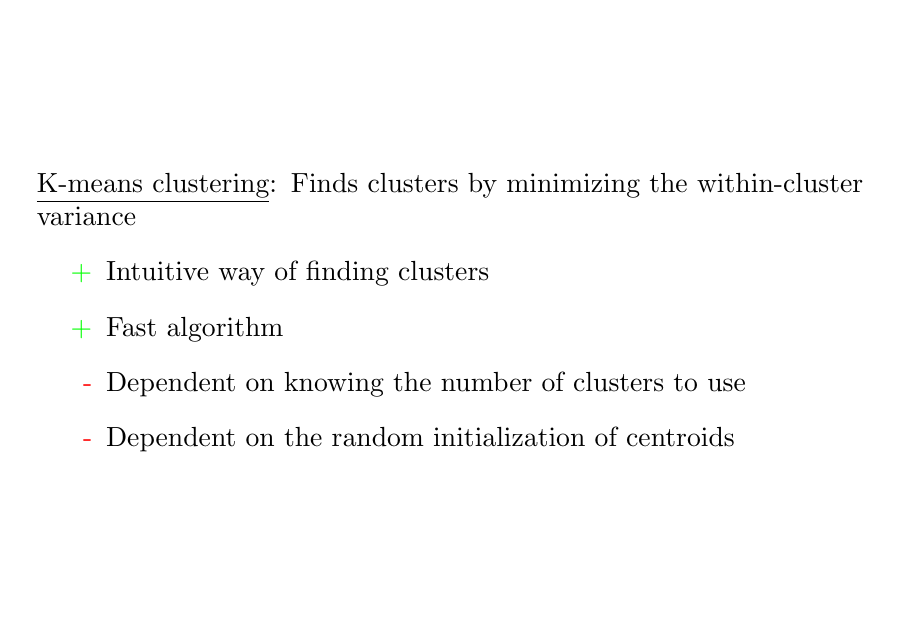
\begin{tikzpicture}
        \node[] at (-5.25, 3.5) {};
        \node[] at (-5.25, -3.5) {};

        \node[text width=10.5cm] at (0, 0) {
            \underline{K-means clustering}: Finds clusters by minimizing the within-cluster variance
            \begin{itemize}
                \item[\textcolor{green}{+}] Intuitive way of finding clusters
                \item[\textcolor{green}{+}] Fast algorithm
                \item[\textcolor{red}{-}] Dependent on knowing the number of clusters to use
                \item[\textcolor{red}{-}] Dependent on the random initialization of centroids
            \end{itemize}
        };
    \end{tikzpicture}
\end{frame}

\newcommand{\hierchicalplot}[1]{
    \begin{tikzpicture}
        \begin{axis}[
            height=5.5cm,
            width=5.5cm,
            xmajorticks=false,
            ymajorticks=false,
            xlabel=$x_1$,
            ylabel=$x_2$,
            xmin=-0.11,
            xmax=0.25,
            ymin=-0.205,
            ymax=0.21
        ]
            \addplot[
                only marks,
                blue,
                opacity=0.5
            ] coordinates {
                (-0.025, -0.056) %0
                (-0.017, 0.026) %1
                (-0.061, -0.061) %2
                (0.028, -0.011) %3
                (-0.073, -0.022) %4
                (0.126, 0.126) %5
                (0.162, 0.054) %6
                (0.063, 0.121) %7
                (0.099, 0.165) %8
                (0.104, 0.079) %9
                (0.223, -0.094) %10
                (0.138, -0.157) %11
                (0.153, -0.081) %12
                (0.078, -0.13) %13
                (0.122, -0.114) %14
            };

            \ifnum#1=1
                \node[anchor=east, font=\tiny, inner sep=2pt] at (axis cs: -0.025, -0.056) {0};
                \node[anchor=east, font=\tiny, inner sep=2pt] at (axis cs: -0.017, 0.026) {1};
                \node[anchor=east, font=\tiny, inner sep=2pt] at (axis cs: -0.061, -0.061) {2};
                \node[anchor=east, font=\tiny, inner sep=2pt] at (axis cs: 0.028, -0.011) {3};
                \node[anchor=east, font=\tiny, inner sep=2pt] at (axis cs: -0.073, -0.022) {4};
                \node[anchor=east, font=\tiny, inner sep=2pt] at (axis cs: 0.126, 0.126) {5};
                \node[anchor=east, font=\tiny, inner sep=2pt] at (axis cs: 0.162, 0.054) {6};
                \node[anchor=east, font=\tiny, inner sep=2pt] at (axis cs: 0.063, 0.121) {7};
                \node[anchor=east, font=\tiny, inner sep=2pt] at (axis cs: 0.099, 0.165) {8};
                \node[anchor=east, font=\tiny, inner sep=2pt] at (axis cs: 0.104, 0.079) {9};
                \node[anchor=east, font=\tiny, inner sep=2pt] at (axis cs: 0.223, -0.094) {10};
                \node[anchor=east, font=\tiny, inner sep=2pt] at (axis cs: 0.138, -0.157) {11};
                \node[anchor=east, font=\tiny, inner sep=2pt] at (axis cs: 0.153, -0.081) {12};
                \node[anchor=east, font=\tiny, inner sep=2pt] at (axis cs: 0.078, -0.13) {13};
                \node[anchor=east, font=\tiny, inner sep=2pt] at (axis cs: 0.122, -0.114) {14};
            \fi

            \ifnum#1<17
                \ifnum#1=2
                    \draw[red] (axis cs: -0.043, -0.058) ellipse [x radius=0.31cm, y radius=0.13cm, rotate=7];
                \fi
                \ifnum#1>2
                    \draw[] (axis cs: -0.043, -0.058) ellipse [x radius=0.31cm, y radius=0.13cm, rotate=7];
                \fi

                \ifnum#1=3
                    \draw[red] (axis cs: 0.1375, -0.0975) ellipse [x radius=0.35cm, y radius=0.13cm, rotate=43];
                \fi
                \ifnum#1>3
                    \draw[] (axis cs: 0.1375, -0.0975) ellipse [x radius=0.35cm, y radius=0.13cm, rotate=43];
                \fi

                \ifnum#1=4
                    \draw[red] (axis cs: 0.1125, 0.1455) ellipse [x radius=0.38cm, y radius=0.13cm, rotate=128];
                \fi
                \ifnum#1>4
                    \draw[] (axis cs: 0.1125, 0.1455) ellipse [x radius=0.38cm, y radius=0.13cm, rotate=128];
                \fi

                \ifnum#1=5
                    \draw[rounded corners, red] (axis cs: 0.012, -0.065) -- (axis cs: -0.07, -0.079) -- (axis cs: -0.086, -0.002) -- cycle;
                \fi
                \ifnum#1>5
                    \draw[rounded corners] (axis cs: 0.012, -0.065) -- (axis cs: -0.07, -0.079) -- (axis cs: -0.086, -0.002) -- cycle;
                \fi

                \ifnum#1=6
                    \draw[red] (axis cs: 0.0835, 0.1) ellipse [x radius=0.43cm, y radius=0.14cm, rotate=139];
                \fi
                \ifnum#1>6
                    \draw[] (axis cs: 0.0835, 0.1) ellipse [x radius=0.43cm, y radius=0.14cm, rotate=139];
                \fi

                \ifnum#1=7
                    \draw[red] (axis cs: 0.0055, 0.0075) ellipse [x radius=0.44cm, y radius=0.14cm, rotate=144];
                \fi
                \ifnum#1>7
                    \draw[] (axis cs: 0.0055, 0.0075) ellipse [x radius=0.44cm, y radius=0.14cm, rotate=144];
                \fi

                \ifnum#1=8
                    \draw[red] (axis cs: 0.108, -0.1435) ellipse [x radius=0.48cm, y radius=0.15cm, rotate=158];
                \fi
                \ifnum#1>8
                    \draw[] (axis cs: 0.108, -0.1435) ellipse [x radius=0.48cm, y radius=0.15cm, rotate=158];
                \fi

                \ifnum#1=9
                    \draw[rounded corners, red] (axis cs: 0.098, 0.193) -- (axis cs: 0.041, 0.116) -- (axis cs: 0.11, 0.055) -- (axis cs: 0.145, 0.126) -- cycle;
                \fi
                \ifnum#1>9
                    \draw[rounded corners] (axis cs: 0.098, 0.193) -- (axis cs: 0.041, 0.116) -- (axis cs: 0.11, 0.055) -- (axis cs: 0.145, 0.126) -- cycle;
                \fi

                \ifnum#1=10
                    \draw[rounded corners,red] (axis cs: 0.17, -0.055) -- (axis cs: 0.042, -0.135) -- (axis cs: 0.148, -0.18) -- cycle;
                \fi
                \ifnum#1>10
                    \draw[rounded corners] (axis cs: 0.17, -0.055) -- (axis cs: 0.042, -0.135) -- (axis cs: 0.148, -0.18) -- cycle;
                \fi

                \ifnum#1=11
                    \draw[rounded corners,red] (axis cs: 0.099, 0.197) -- (axis cs: 0.035, 0.118) -- (axis cs: 0.105, 0.055) -- (axis cs: 0.177, 0.041) -- (axis cs: 0.15, 0.126) -- cycle;
                \fi
                \ifnum#1>11
                    \draw[rounded corners] (axis cs: 0.099, 0.197) -- (axis cs: 0.035, 0.118) -- (axis cs: 0.105, 0.055) -- (axis cs: 0.177, 0.041) -- (axis cs: 0.15, 0.126) -- cycle;
                \fi

                \ifnum#1=12
                    \draw[rounded corners,red] (axis cs: -0.017, 0.047) -- (axis cs: -0.09, -0.005) -- (axis cs: -0.072, -0.083) -- (axis cs: 0.007, -0.07) -- (axis cs: 0.05, -0.007) -- cycle;
                \fi
                \ifnum#1>12
                    \draw[rounded corners] (axis cs: -0.017, 0.047) -- (axis cs: -0.09, -0.005) -- (axis cs: -0.072, -0.083) -- (axis cs: 0.007, -0.07) -- (axis cs: 0.05, -0.007) -- cycle;
                \fi

                \ifnum#1=13
                    \draw[rounded corners,red] (axis cs: 0.17, -0.05) -- (axis cs: 0.038, -0.135) -- (axis cs: 0.148, -0.185) -- (axis cs: 0.24, -0.092) -- cycle;
                \fi
                \ifnum#1>13
                    \draw[rounded corners] (axis cs: 0.17, -0.05) -- (axis cs: 0.038, -0.135) -- (axis cs: 0.148, -0.185) -- (axis cs: 0.24, -0.092) -- cycle;
                \fi

                \ifnum#1=14
                    \draw[rounded corners, red] (axis cs: 0.17, -0.045) -- (axis cs: -0.017, 0.05) -- (axis cs: -0.095, -0.005) -- (axis cs: -0.077, -0.083) -- (axis cs: 0.042, -0.14) -- (axis cs: 0.148, -0.19) -- (axis cs: 0.245, -0.092) -- cycle;
                \fi
                \ifnum#1>14
                    \draw[rounded corners] (axis cs: 0.17, -0.045) -- (axis cs: -0.017, 0.05) -- (axis cs: -0.095, -0.005) -- (axis cs: -0.077, -0.083) -- (axis cs: 0.042, -0.14) -- (axis cs: 0.148, -0.19) -- (axis cs: 0.245, -0.092) -- cycle;
                \fi

                \ifnum#1=15
                    \draw[rounded corners, red] (axis cs: 0.099, 0.2) -- (axis cs: -0.1, -0.005) -- (axis cs: -0.082, -0.083) -- (axis cs: 0.042, -0.145) -- (axis cs: 0.148, -0.195) -- (axis cs: 0.25, -0.092) -- (axis cs: 0.155, 0.126) -- cycle;
                \fi
                \ifnum#1>15
                    \draw[rounded corners] (axis cs: 0.099, 0.2) -- (axis cs: -0.1, -0.005) -- (axis cs: -0.082, -0.083) -- (axis cs: 0.042, -0.145) -- (axis cs: 0.148, -0.195) -- (axis cs: 0.25, -0.092) -- (axis cs: 0.155, 0.126) -- cycle;
                \fi
            \fi
            \ifnum#1=17
                \draw[rounded corners,red] (axis cs: 0.17, -0.055) -- (axis cs: 0.042, -0.135) -- (axis cs: 0.148, -0.18) -- cycle;
                \draw[rounded corners, red] (axis cs: 0.098, 0.193) -- (axis cs: 0.041, 0.116) -- (axis cs: 0.11, 0.055) -- (axis cs: 0.145, 0.126) -- cycle;
                \draw[red] (axis cs: 0.0055, 0.0075) ellipse [x radius=0.44cm, y radius=0.14cm, rotate=144];
                \draw[rounded corners, red] (axis cs: 0.012, -0.065) -- (axis cs: -0.07, -0.079) -- (axis cs: -0.086, -0.002) -- cycle;
                \draw[red] (axis cs: 0.162, 0.054) ellipse [x radius=0.12cm, y radius=0.12cm];
                \draw[red] (axis cs: 0.223, -0.094) ellipse [x radius=0.12cm, y radius=0.12cm];
            \fi
            \ifnum#1=18
                \draw[rounded corners,red] (axis cs: 0.17, -0.05) -- (axis cs: 0.038, -0.135) -- (axis cs: 0.148, -0.185) -- (axis cs: 0.24, -0.092) -- cycle;
                \draw[rounded corners,red] (axis cs: -0.017, 0.047) -- (axis cs: -0.09, -0.005) -- (axis cs: -0.072, -0.083) -- (axis cs: 0.007, -0.07) -- (axis cs: 0.05, -0.007) -- cycle;
                \draw[rounded corners,red] (axis cs: 0.099, 0.197) -- (axis cs: 0.035, 0.118) -- (axis cs: 0.105, 0.055) -- (axis cs: 0.177, 0.041) -- (axis cs: 0.15, 0.126) -- cycle;
            \fi
            \ifnum#1<21
                \ifnum#1>18
                    \draw[stealth-stealth, red] (axis cs: -0.017, 0.026) --
                    (axis cs: 0.028, -0.011);
                \fi
                \ifnum#1=20
                    \draw[stealth-stealth] (axis cs: -0.017, 0.026) --
                    (axis cs: -0.017, -0.011) -- (axis cs: 0.028, -0.011);
                \fi
            \fi
            \ifnum#1=21
                \draw[] (axis cs: 0.1125, 0.1455) ellipse [x radius=0.38cm, y radius=0.13cm, rotate=128];
                \draw[] (axis cs: 0.0835, 0.1) ellipse [x radius=0.43cm, y radius=0.14cm, rotate=139];
                \draw[stealth-stealth, red] (axis cs: 0.1125, 0.1455) -- (axis cs: 0.0835, 0.1);
            \fi
        \end{axis}
    \end{tikzpicture}
}

\newsavebox{\hierarchicaldata}
\sbox{\hierarchicaldata}{
    \hierchicalplot{0}
}
\newsavebox{\hierarchicalids}
\sbox{\hierarchicalids}{
    \hierchicalplot{1}
}
\newsavebox{\hierarchicalfirst}
\sbox{\hierarchicalfirst}{
    \hierchicalplot{2}
}
\newsavebox{\hierarchicalsecond}
\sbox{\hierarchicalsecond}{
    \hierchicalplot{3}
}
\newsavebox{\hierarchicalthird}
\sbox{\hierarchicalthird}{
    \hierchicalplot{4}
}
\newsavebox{\hierarchicalfourth}
\sbox{\hierarchicalfourth}{
    \hierchicalplot{5}
}
\newsavebox{\hierarchicalfifth}
\sbox{\hierarchicalfifth}{
    \hierchicalplot{6}
}
\newsavebox{\hierarchicalsixth}
\sbox{\hierarchicalsixth}{
    \hierchicalplot{7}
}
\newsavebox{\hierarchicalseventh}
\sbox{\hierarchicalseventh}{
    \hierchicalplot{8}
}
\newsavebox{\hierarchicaleight}
\sbox{\hierarchicaleight}{
    \hierchicalplot{9}
}
\newsavebox{\hierarchicalninth}
\sbox{\hierarchicalninth}{
    \hierchicalplot{10}
}
\newsavebox{\hierarchicaltenth}
\sbox{\hierarchicaltenth}{
    \hierchicalplot{11}
}
\newsavebox{\hierarchicaleleventh}
\sbox{\hierarchicaleleventh}{
    \hierchicalplot{12}
}
\newsavebox{\hierarchicaltwelfth}
\sbox{\hierarchicaltwelfth}{
    \hierchicalplot{13}
}
\newsavebox{\hierarchicalthirteenth}
\sbox{\hierarchicalthirteenth}{
    \hierchicalplot{14}
}
\newsavebox{\hierarchicalfourteenth}
\sbox{\hierarchicalfourteenth}{
    \hierchicalplot{15}
}
\newsavebox{\hierarchicalfull}
\sbox{\hierarchicalfull}{
    \hierchicalplot{16}
}
\newsavebox{\hierarchicalfirstthreshold}
\sbox{\hierarchicalfirstthreshold}{
    \hierchicalplot{17}
}
\newsavebox{\hierarchicalsecondthreshold}
\sbox{\hierarchicalsecondthreshold}{
    \hierchicalplot{18}
}
\newsavebox{\hierarchicaldistance}
\sbox{\hierarchicaldistance}{
    \hierchicalplot{19}
}
\newsavebox{\hierarchicaleuclidean}
\sbox{\hierarchicaleuclidean}{
    \hierchicalplot{20}
}
\newsavebox{\hierarchicaldissimilarity}
\sbox{\hierarchicaldissimilarity}{
    \hierchicalplot{21}
}

\newcommand{\dendroplot}[1]{
    \begin{tikzpicture}
        \begin{axis}[
            height=5.5cm,
            width=5.5cm,
            xtick pos=bottom,
            ytick pos=left,
            xmin=-0.5,
            xmax=14.5,
            ymin=0,
            ymax=0.5,
            xtick={0, 1, 2, 3, 4, 5, 6, 7, 8, 9, 10, 11, 12, 13, 14},
            xticklabels={6, 5, 8, 7, 9, 4, 0, 2, 1, 3, 10, 12, 14, 11, 13},
            xtick style={draw=none},
            xticklabel style={font=\scriptsize},
            clip=false
        ]
            \ifnum#1=1
                \draw[thick,red] (axis cs: 6, 0) -- (axis cs: 6, 0.036) -- (axis cs: 7, 0.036) -- (axis cs: 7, 0);
            \fi
            \ifnum#1>1
                \draw[thick] (axis cs: 6, 0) -- (axis cs: 6, 0.036) -- (axis cs: 7, 0.036) -- (axis cs: 7, 0);
            \fi

            \ifnum#1=2
                \draw[thick,red] (axis cs: 11, 0) -- (axis cs: 11, 0.045) -- (axis cs: 12, 0.045) -- (axis cs: 12, 0);
            \fi
            \ifnum#1>2
                \draw[thick] (axis cs: 11, 0) -- (axis cs: 11, 0.045) -- (axis cs: 12, 0.045) -- (axis cs: 12, 0);
            \fi

            \ifnum#1=3
                \draw[thick,red] (axis cs: 1, 0) -- (axis cs: 1, 0.047) -- (axis cs: 2, 0.047) -- (axis cs: 2, 0);
            \fi
            \ifnum#1>3
                \draw[thick] (axis cs: 1, 0) -- (axis cs: 1, 0.047) -- (axis cs: 2, 0.047) -- (axis cs: 2, 0);
            \fi

            \ifnum#1=4
                \draw[thick,red] (axis cs: 6.5, 0.036) -- (axis cs: 6.5, 0.054) -- (axis cs: 5, 0.054) -- (axis cs: 5, 0);
            \fi
            \ifnum#1>4
                \draw[thick] (axis cs: 6.5, 0.036) -- (axis cs: 6.5, 0.054) -- (axis cs: 5, 0.054) -- (axis cs: 5, 0);
            \fi

            \ifnum#1=5
                \draw[thick,red] (axis cs: 3, 0) -- (axis cs: 3, 0.058) -- (axis cs: 4, 0.058) -- (axis cs: 4, 0);
            \fi
            \ifnum#1>5
                \draw[thick] (axis cs: 3, 0) -- (axis cs: 3, 0.058) -- (axis cs: 4, 0.058) -- (axis cs: 4, 0);
            \fi

            \ifnum#1=6
                \draw[thick,red] (axis cs: 8, 0) -- (axis cs: 8, 0.059) -- (axis cs: 9, 0.059) -- (axis cs: 9, 0);
            \fi
            \ifnum#1>6
                \draw[thick] (axis cs: 8, 0) -- (axis cs: 8, 0.059) -- (axis cs: 9, 0.059) -- (axis cs: 9, 0);
            \fi

            \ifnum#1=7
                \draw[thick,red] (axis cs: 13, 0) -- (axis cs: 13, 0.065) -- (axis cs: 14, 0.065) -- (axis cs: 14, 0);
            \fi
            \ifnum#1>7
                \draw[thick] (axis cs: 13, 0) -- (axis cs: 13, 0.065) -- (axis cs: 14, 0.065) -- (axis cs: 14, 0);
            \fi

            \ifnum#1=8
                \draw[thick,red] (axis cs: 1.5, 0.047) -- (axis cs: 1.5, 0.076) -- (axis cs: 3.5, 0.076) -- (axis cs: 3.5, 0.058);
            \fi
            \ifnum#1>8
                \draw[thick] (axis cs: 1.5, 0.047) -- (axis cs: 1.5, 0.076) -- (axis cs: 3.5, 0.076) -- (axis cs: 3.5, 0.058);
            \fi

            \ifnum#1=9
                \draw[thick,red] (axis cs: 11.5, 0.045) -- (axis cs: 11.5, 0.077) -- (axis cs: 13.5, 0.077) -- (axis cs: 13.5, 0.065);
            \fi
            \ifnum#1>9
                \draw[thick] (axis cs: 11.5, 0.045) -- (axis cs: 11.5, 0.077) -- (axis cs: 13.5, 0.077) -- (axis cs: 13.5, 0.065);
            \fi

            \ifnum#1=10
                \draw[thick,red] (axis cs: 2.5, 0.076) -- (axis cs: 2.5, 0.118) -- (axis cs: 0, 0.118) -- (axis cs: 0, 0);
            \fi
            \ifnum#1>10
                \draw[thick] (axis cs: 2.5, 0.076) -- (axis cs: 2.5, 0.118) -- (axis cs: 0, 0.118) -- (axis cs: 0, 0);
            \fi

            \ifnum#1=11
                \draw[thick,red] (axis cs: 6, 0.054) -- (axis cs: 6, 0.124) -- (axis cs: 8.5, 0.124) -- (axis cs: 8.5, 0.059);
            \fi
            \ifnum#1>11
                \draw[thick] (axis cs: 6, 0.054) -- (axis cs: 6, 0.124) -- (axis cs: 8.5, 0.124) -- (axis cs: 8.5, 0.059);
            \fi

            \ifnum#1=12
                \draw[thick,red] (axis cs: 12.5, 0.077) -- (axis cs: 12.5, 0.130) -- (axis cs: 10, 0.130) -- (axis cs: 10, 0);
            \fi
            \ifnum#1>12
                \draw[thick] (axis cs: 12.5, 0.077) -- (axis cs: 12.5, 0.130) -- (axis cs: 10, 0.130) -- (axis cs: 10, 0);
            \fi

            \ifnum#1=13
                \draw[thick,red] (axis cs: 11.25, 0.130) -- (axis cs: 11.25, 0.436) -- (axis cs: 7.25, 0.436) -- (axis cs: 7.25, 0.124);
            \fi
            \ifnum#1>13
                \draw[thick] (axis cs: 11.25, 0.130) -- (axis cs: 11.25, 0.436) -- (axis cs: 7.25, 0.436) -- (axis cs: 7.25, 0.124);
            \fi

            \ifnum#1=14
                \draw[thick,red] (axis cs: 9.25, 0.436) -- (axis cs: 9.25, 0.485) -- (axis cs: 1.75, 0.485) -- (axis cs: 1.75, 0.118);
            \fi
            \ifnum#1>14
                \draw[thick] (axis cs: 9.25, 0.436) -- (axis cs: 9.25, 0.485) -- (axis cs: 1.75, 0.485) -- (axis cs: 1.75, 0.118);
            \fi
            \ifnum#1=16
                \draw[very thick, red] (axis cs: -0.5, 0.1) -- (axis cs: 14.5, 0.1);
            \fi
            \ifnum#1=17
                \draw[very thick, red] (axis cs: -0.5, 0.3) -- (axis cs: 14.5, 0.3);
            \fi
            \ifnum#1=18
                \draw[very thick, stealth-stealth, red] (axis cs: -0.5, 0) -- (axis cs: -0.5, 0.5);
            \fi
        \end{axis}
    \end{tikzpicture}
}

\newsavebox{\dendroinit}
\sbox{\dendroinit}{
    \dendroplot{0}
}
\newsavebox{\dendrofirst}
\sbox{\dendrofirst}{
    \dendroplot{1}
}
\newsavebox{\dendrosecond}
\sbox{\dendrosecond}{
    \dendroplot{2}
}
\newsavebox{\dendrothird}
\sbox{\dendrothird}{
    \dendroplot{3}
}
\newsavebox{\dendrofourth}
\sbox{\dendrofourth}{
    \dendroplot{4}
}
\newsavebox{\dendrofifth}
\sbox{\dendrofifth}{
    \dendroplot{5}
}
\newsavebox{\dendrosixth}
\sbox{\dendrosixth}{
    \dendroplot{6}
}
\newsavebox{\dendroseventh}
\sbox{\dendroseventh}{
    \dendroplot{7}
}
\newsavebox{\dendroeight}
\sbox{\dendroeight}{
    \dendroplot{8}
}
\newsavebox{\dendroninth}
\sbox{\dendroninth}{
    \dendroplot{9}
}
\newsavebox{\dendrotenth}
\sbox{\dendrotenth}{
    \dendroplot{10}
}
\newsavebox{\dendroeleventh}
\sbox{\dendroeleventh}{
    \dendroplot{11}
}
\newsavebox{\dendrotwelfth}
\sbox{\dendrotwelfth}{
    \dendroplot{12}
}
\newsavebox{\dendrothirteenth}
\sbox{\dendrothirteenth}{
    \dendroplot{13}
}
\newsavebox{\dendrofourteenth}
\sbox{\dendrofourteenth}{
    \dendroplot{14}
}
\newsavebox{\dendrofull}
\sbox{\dendrofull}{
    \dendroplot{15}
}
\newsavebox{\dendrofirstthreshold}
\sbox{\dendrofirstthreshold}{
    \dendroplot{16}
}
\newsavebox{\dendrosecondthreshold}
\sbox{\dendrosecondthreshold}{
    \dendroplot{17}
}
\newsavebox{\dendroheight}
\sbox{\dendroheight}{
    \dendroplot{18}
}

\begin{frame}{Hierarchical clustering: Algorithm}
    \begin{tikzpicture}
        \node[] at (-5.25, 3.5) {};
        \node[] at (-5.25, -3.5) {};

        \visible<1>{
            \node[anchor=north east] at (5.25, 2.5) {
                \usebox{\hierarchicaldata}
            };
        }
        \visible<2-3>{
            \node[anchor=north east] at (5.25, 2.5) {
                \usebox{\hierarchicalids}
            };
        }
        \visible<3>{
            \node[anchor=north west] at (-5.25, 2.5) {
                \usebox{\dendroinit}
            };
        }
        \visible<4>{
            \node[anchor=north west] at (-5.25, 2.5) {
                \usebox{\dendrofirst}
            };
            \node[anchor=north east] at (5.25, 2.5) {
                \usebox{\hierarchicalfirst}
            };
        }
        \visible<5>{
            \node[anchor=north west] at (-5.25, 2.5) {
                \usebox{\dendrosecond}
            };
            \node[anchor=north east] at (5.25, 2.5) {
                \usebox{\hierarchicalsecond}
            };
        }
        \visible<6>{
            \node[anchor=north west] at (-5.25, 2.5) {
                \usebox{\dendrothird}
            };
            \node[anchor=north east] at (5.25, 2.5) {
                \usebox{\hierarchicalthird}
            };
        }
        \visible<7>{
            \node[anchor=north west] at (-5.25, 2.5) {
                \usebox{\dendrofourth}
            };
            \node[anchor=north east] at (5.25, 2.5) {
                \usebox{\hierarchicalfourth}
            };
        }
        \visible<8>{
            \node[anchor=north west] at (-5.25, 2.5) {
                \usebox{\dendrofifth}
            };
            \node[anchor=north east] at (5.25, 2.5) {
                \usebox{\hierarchicalfifth}
            };
        }
        \visible<9>{
            \node[anchor=north west] at (-5.25, 2.5) {
                \usebox{\dendrosixth}
            };
            \node[anchor=north east] at (5.25, 2.5) {
                \usebox{\hierarchicalsixth}
            };
        }
        \visible<10>{
            \node[anchor=north west] at (-5.25, 2.5) {
                \usebox{\dendroseventh}
            };
            \node[anchor=north east] at (5.25, 2.5) {
                \usebox{\hierarchicalseventh}
            };
        }
        \visible<11>{
            \node[anchor=north west] at (-5.25, 2.5) {
                \usebox{\dendroeight}
            };
            \node[anchor=north east] at (5.25, 2.5) {
                \usebox{\hierarchicaleight}
            };
        }
        \visible<12>{
            \node[anchor=north west] at (-5.25, 2.5) {
                \usebox{\dendroninth}
            };
            \node[anchor=north east] at (5.25, 2.5) {
                \usebox{\hierarchicalninth}
            };
        }
        \visible<13>{
            \node[anchor=north west] at (-5.25, 2.5) {
                \usebox{\dendrotenth}
            };
            \node[anchor=north east] at (5.25, 2.5) {
                \usebox{\hierarchicaltenth}
            };
        }
        \visible<14>{
            \node[anchor=north west] at (-5.25, 2.5) {
                \usebox{\dendroeleventh}
            };
            \node[anchor=north east] at (5.25, 2.5) {
                \usebox{\hierarchicaleleventh}
            };
        }
        \visible<15>{
            \node[anchor=north west] at (-5.25, 2.5) {
                \usebox{\dendrotwelfth}
            };
            \node[anchor=north east] at (5.25, 2.5) {
                \usebox{\hierarchicaltwelfth}
            };
        }
        \visible<16>{
            \node[anchor=north west] at (-5.25, 2.5) {
                \usebox{\dendrothirteenth}
            };
            \node[anchor=north east] at (5.25, 2.5) {
                \usebox{\hierarchicalthirteenth}
            };
        }
        \visible<17>{
            \node[anchor=north west] at (-5.25, 2.5) {
                \usebox{\dendrofourteenth}
            };
            \node[anchor=north east] at (5.25, 2.5) {
                \usebox{\hierarchicalfourteenth}
            };
        }
        \visible<18>{
            \node[anchor=north west] at (-5.25, 2.5) {
                \usebox{\dendrofull}
            };
            \node[anchor=north east] at (5.25, 2.5) {
                \usebox{\hierarchicalfull}
            };
        }
    \end{tikzpicture}
\end{frame}

\begin{frame}{Hierarchical clustering: Interpretation}
    \begin{tikzpicture}
        \node[] at (-5.25, 3.5) {};
        \node[] at (-5.25, -3.5) {};

        \visible<1>{
            \node[anchor=north west] at (-5.25, 2.5) {
                \usebox{\dendrofirstthreshold}
            };
            \node[anchor=north east] at (5.25, 2.5) {
                \usebox{\hierarchicalfirstthreshold}
            };
        }
        \visible<2,4>{
            \node[anchor=north west] at (-5.25, 2.5) {
                \usebox{\dendrosecondthreshold}
            };
            \node[anchor=north east] at (5.25, 2.5) {
                \usebox{\hierarchicalsecondthreshold}
            };
        }
        \visible<3>{
            \node[anchor=north west] at (-5.25, 2.5) {
                \usebox{\dendroheight}
            };
            \node[anchor=north east] at (5.25, 2.5) {
                \usebox{\hierarchicaldata}
            };
        }
        \visible<5-7>{
            \node[anchor=north west] at (-5.25, 2.5) {
                \usebox{\dendrofull}
            };
        }
        \visible<5>{
            \node[anchor=north east] at (5.25, 2.5) {
                \usebox{\hierarchicaldistance}
            };
        }
        \visible<6>{
            \node[anchor=north east] at (5.25, 2.5) {
                \usebox{\hierarchicaleuclidean}
            };
        }
        \visible<7-8>{
            \node[anchor=north east] at (5.25, 2.5) {
                \usebox{\hierarchicaldissimilarity}
            };
        }
        \visible<8>{
            \node[anchor=north west] at (-5.25, 2.5) {
                \usebox{\dendroheight}
            };
        }
        \visible<9>{
            \node[] at (0, 0) {
                \begin{tabular}{|m{2cm}|p{6.1cm}|}
                    \hline
                    Complete&Maximal intercluster dissimilarity\\
                    \hline
                    Single&Minimal intercluster dissimilarity\\
                    \hline
                    Average&Mean intercluster dissimilarity\\
                    \hline
                    Centroid&Dissimilarity between the centroid for cluster A and the centroid for cluster B.\\
                    \hline
                \end{tabular}
            };
        }
        \visible<10>{
            \node[text width=10.5cm] at (0, 0) {
                \underline{Agglomerative clustering}: Iteratively merge clusters to form a hierarchy of cluster assignments.
                \begin{itemize}
                    \item[\textcolor{green}{+}] Not reliant on \textit{a priori} deciding the number of clusters
                    \item[\textcolor{red}{-}] Still relies on choices: Distance metric, linkage method, threshold
                \end{itemize}
            };
        }
    \end{tikzpicture}
\end{frame}

\section{\emoji{skull-and-crossbones}\emoji{skull-and-crossbones}\emoji{skull-and-crossbones} Clustering horror story \emoji{skull-and-crossbones}\emoji{skull-and-crossbones}\emoji{skull-and-crossbones}}

\begin{frame}{\emoji{skull-and-crossbones}\emoji{skull-and-crossbones}\emoji{skull-and-crossbones} Clustering horror story \emoji{skull-and-crossbones}\emoji{skull-and-crossbones}\emoji{skull-and-crossbones}}
    \centering
    \begin{tikzpicture}
        \visible<1>{
            \node[inner sep=0pt, draw=black] at (0, 0) {
                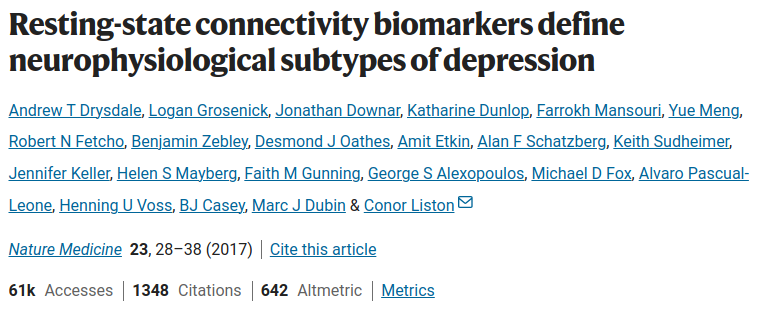
\includegraphics[width=7cm]{data/drysdale.png}
            };
        }
        \visible<2>{
            \node[inner sep=0pt, draw=black] at (0, 0) {
                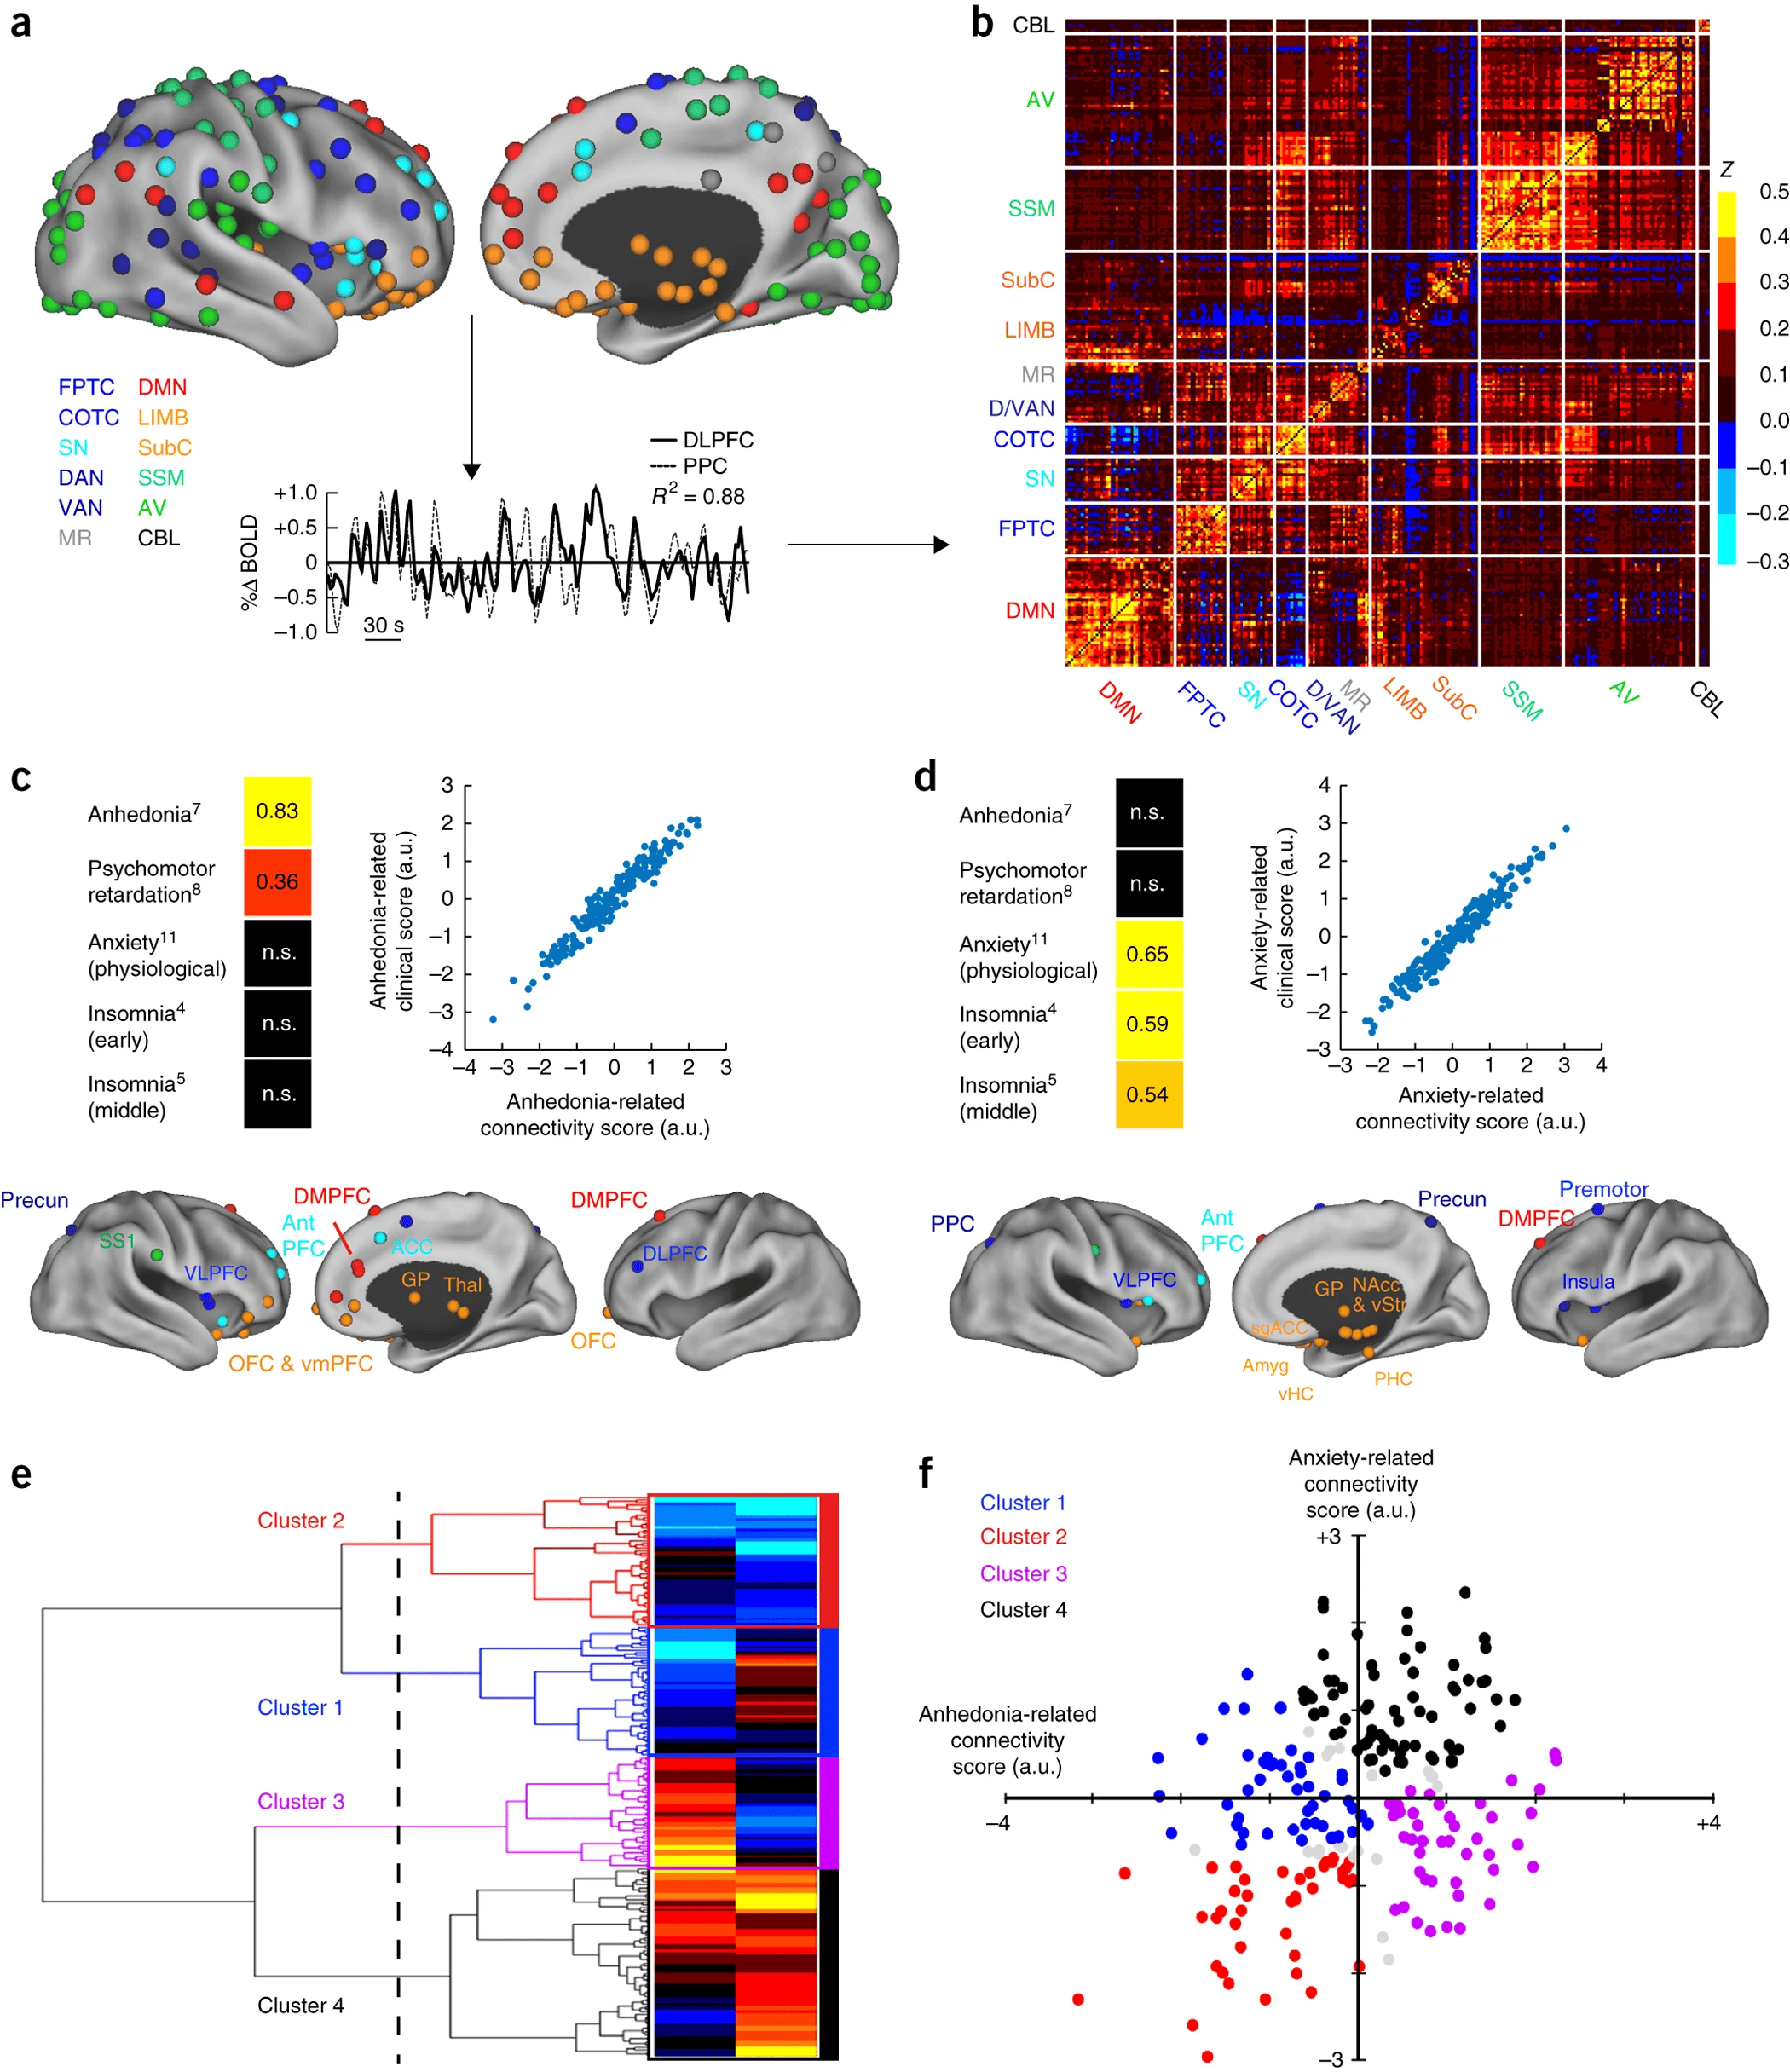
\includegraphics[height=7cm]{data/fig1.png}
            };
        }
        \visible<3>{
            \node[inner sep=0pt, draw=black] at (0, 0) {
                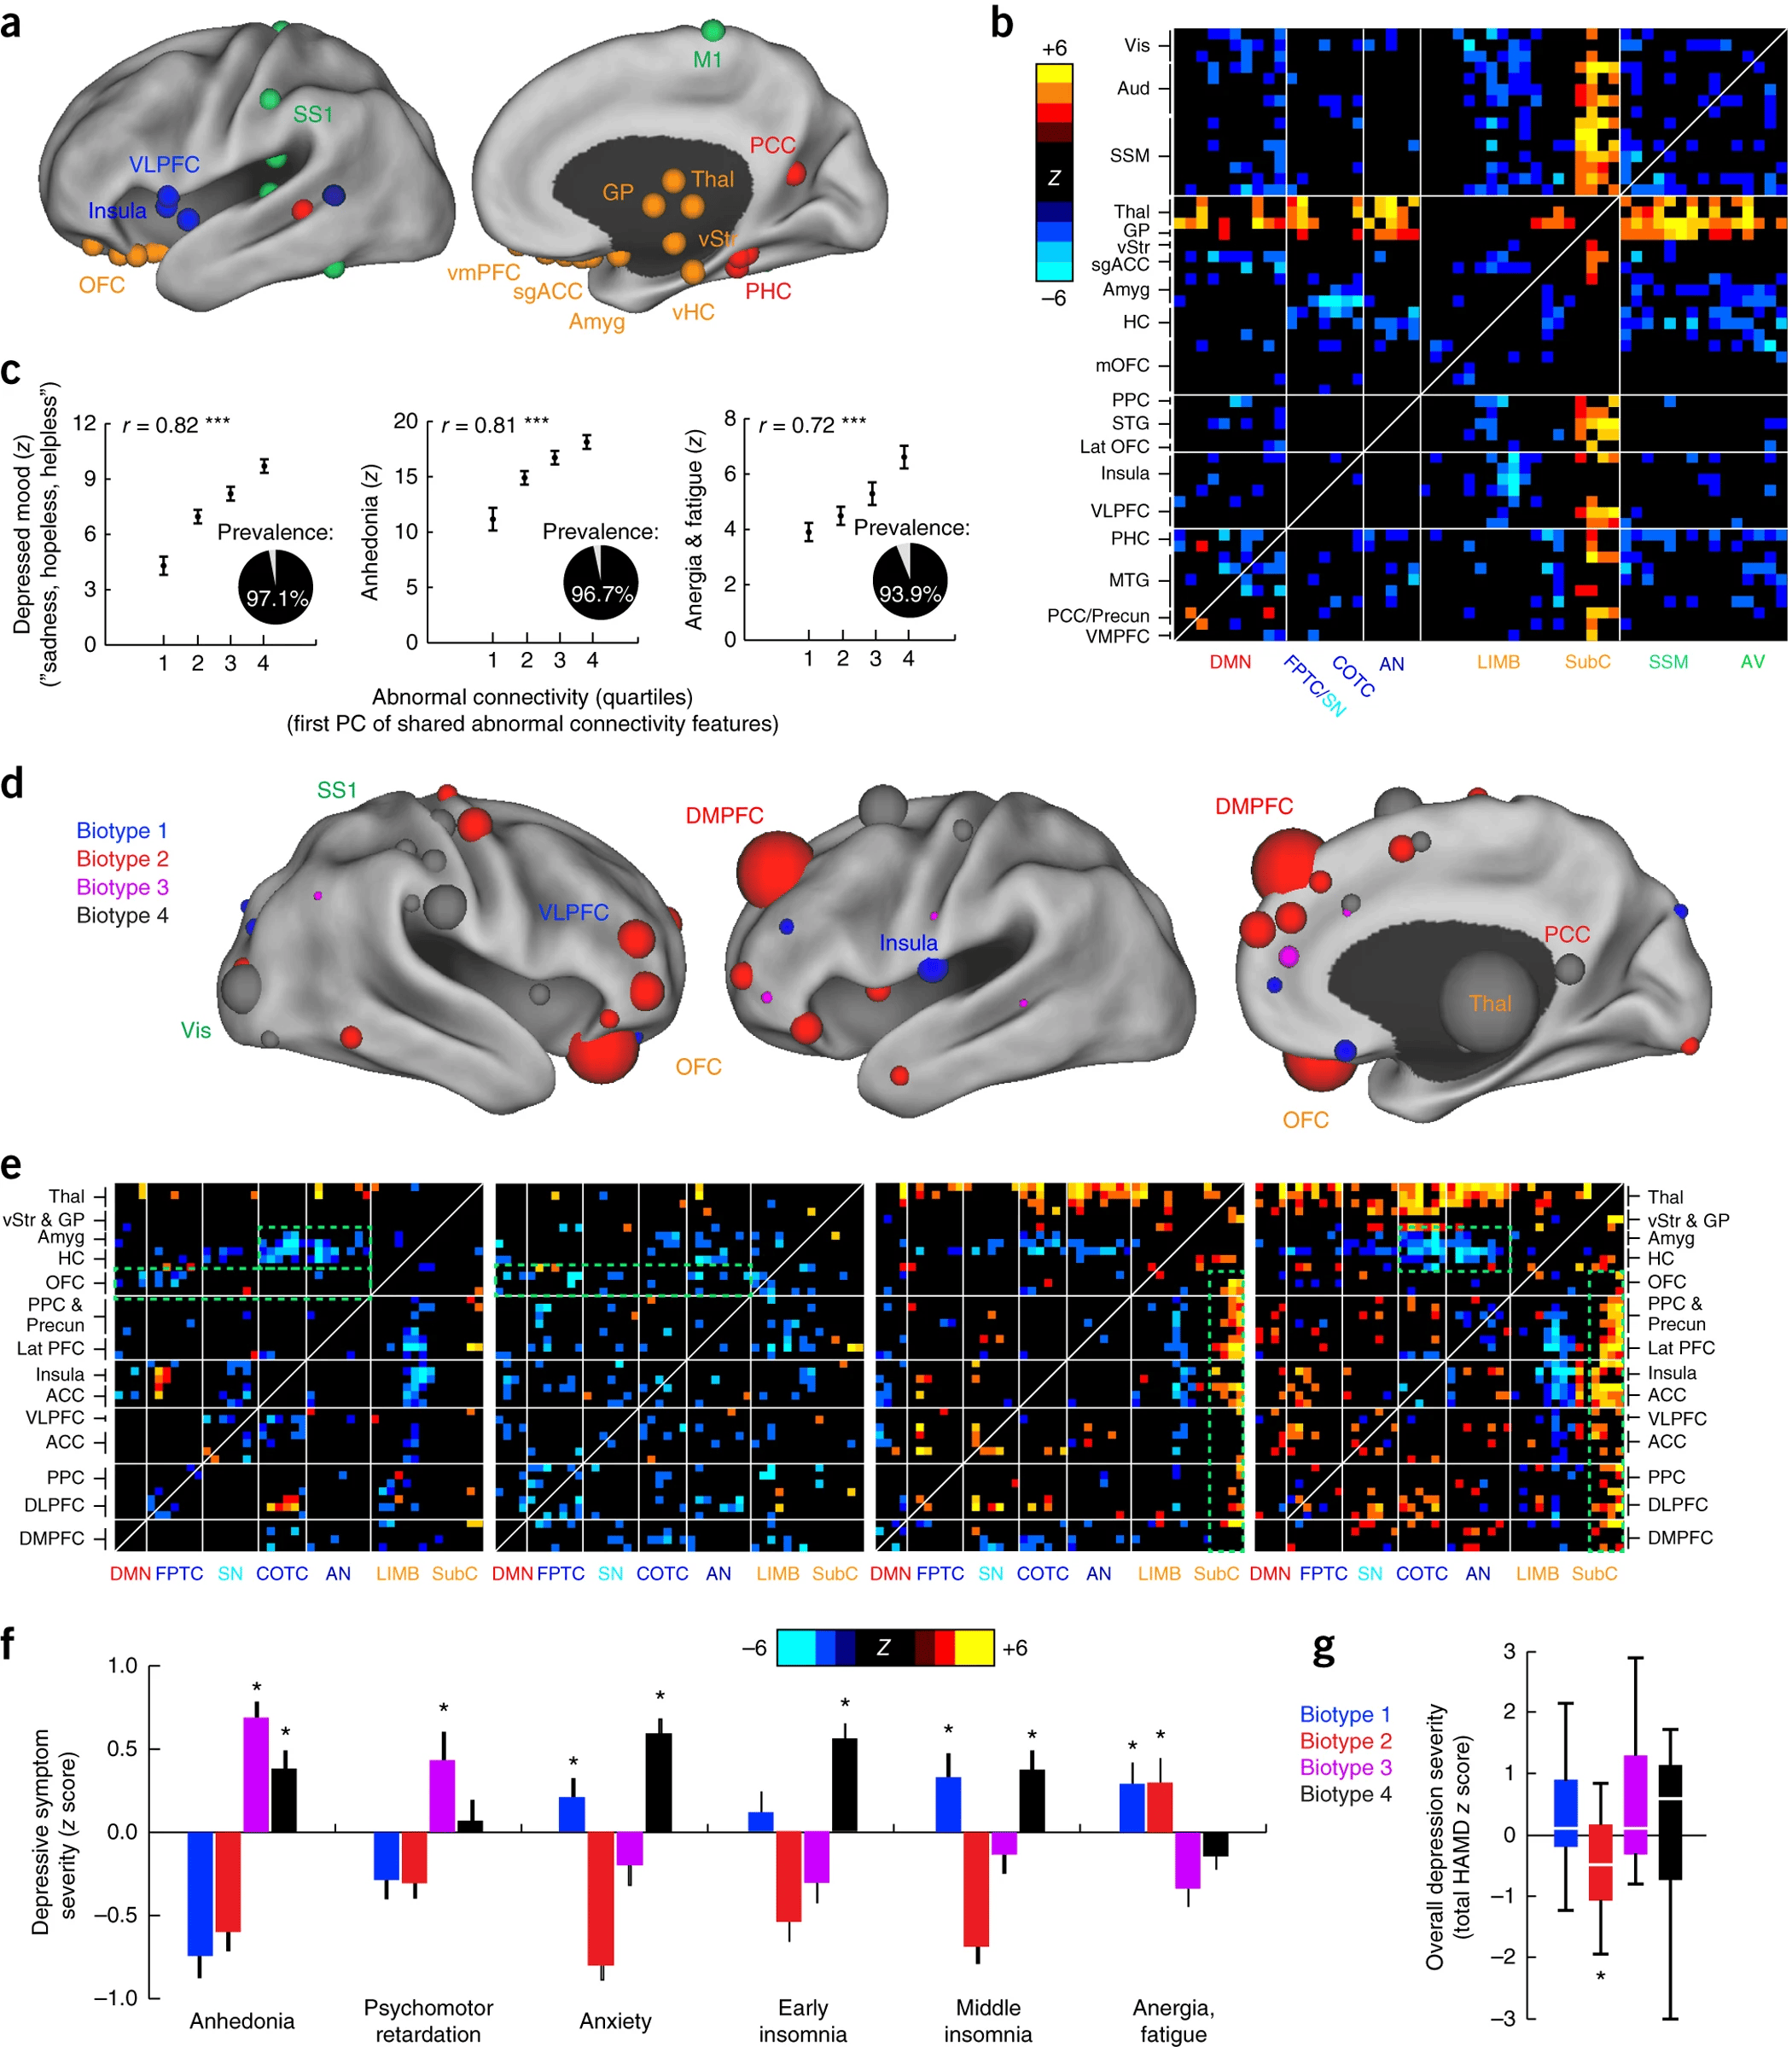
\includegraphics[height=7cm]{data/fig2.png}
            };
        }
        \visible<4>{
            \node[inner sep=0pt, draw=black] at (0, 0) {
                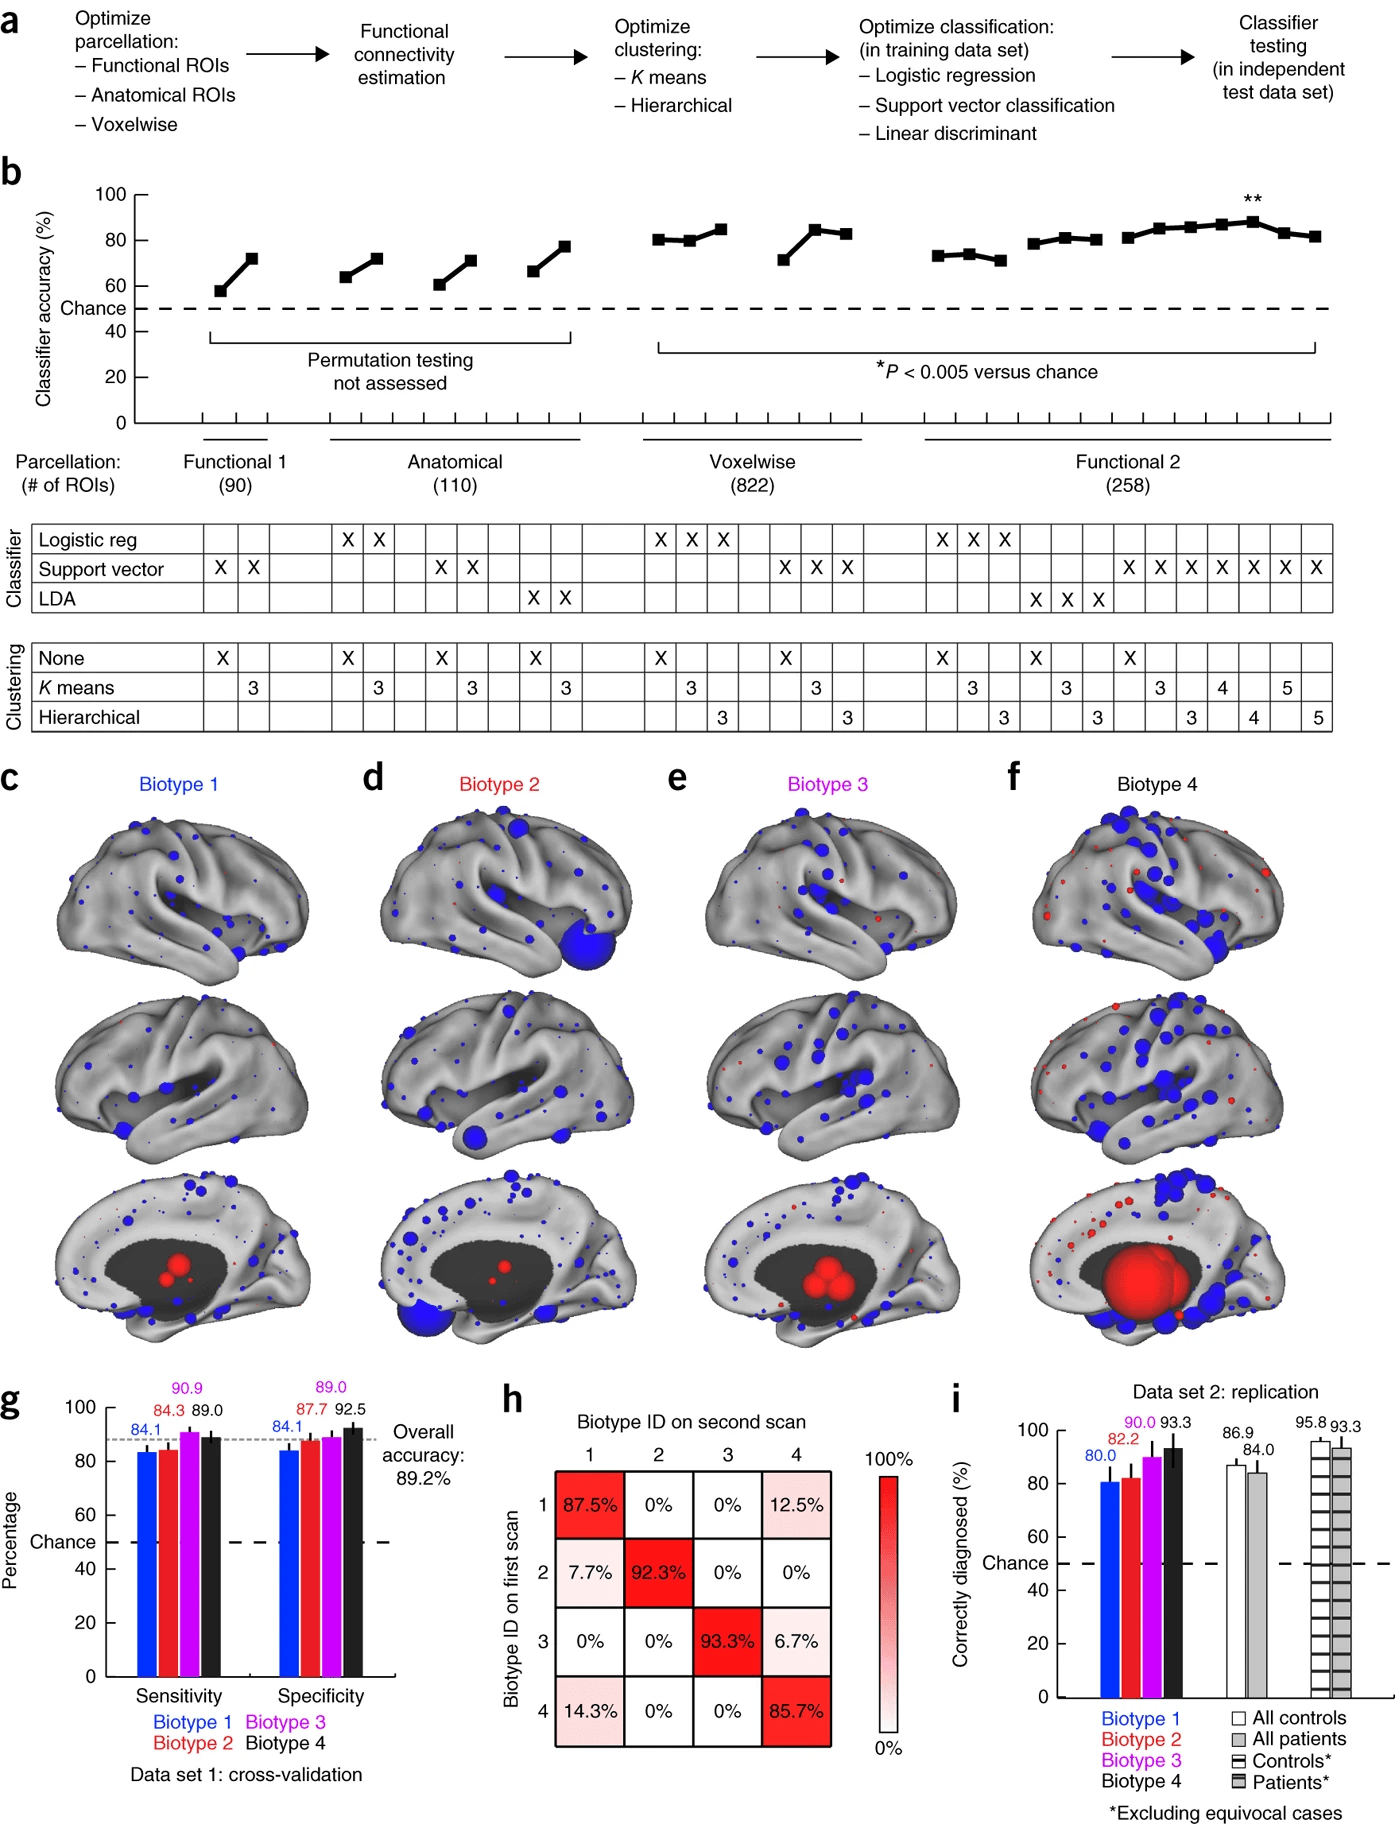
\includegraphics[height=7cm]{data/fig3.png}
            };
        }
        \visible<5>{
            \node[inner sep=0pt, draw=black] at (0, 0) {
                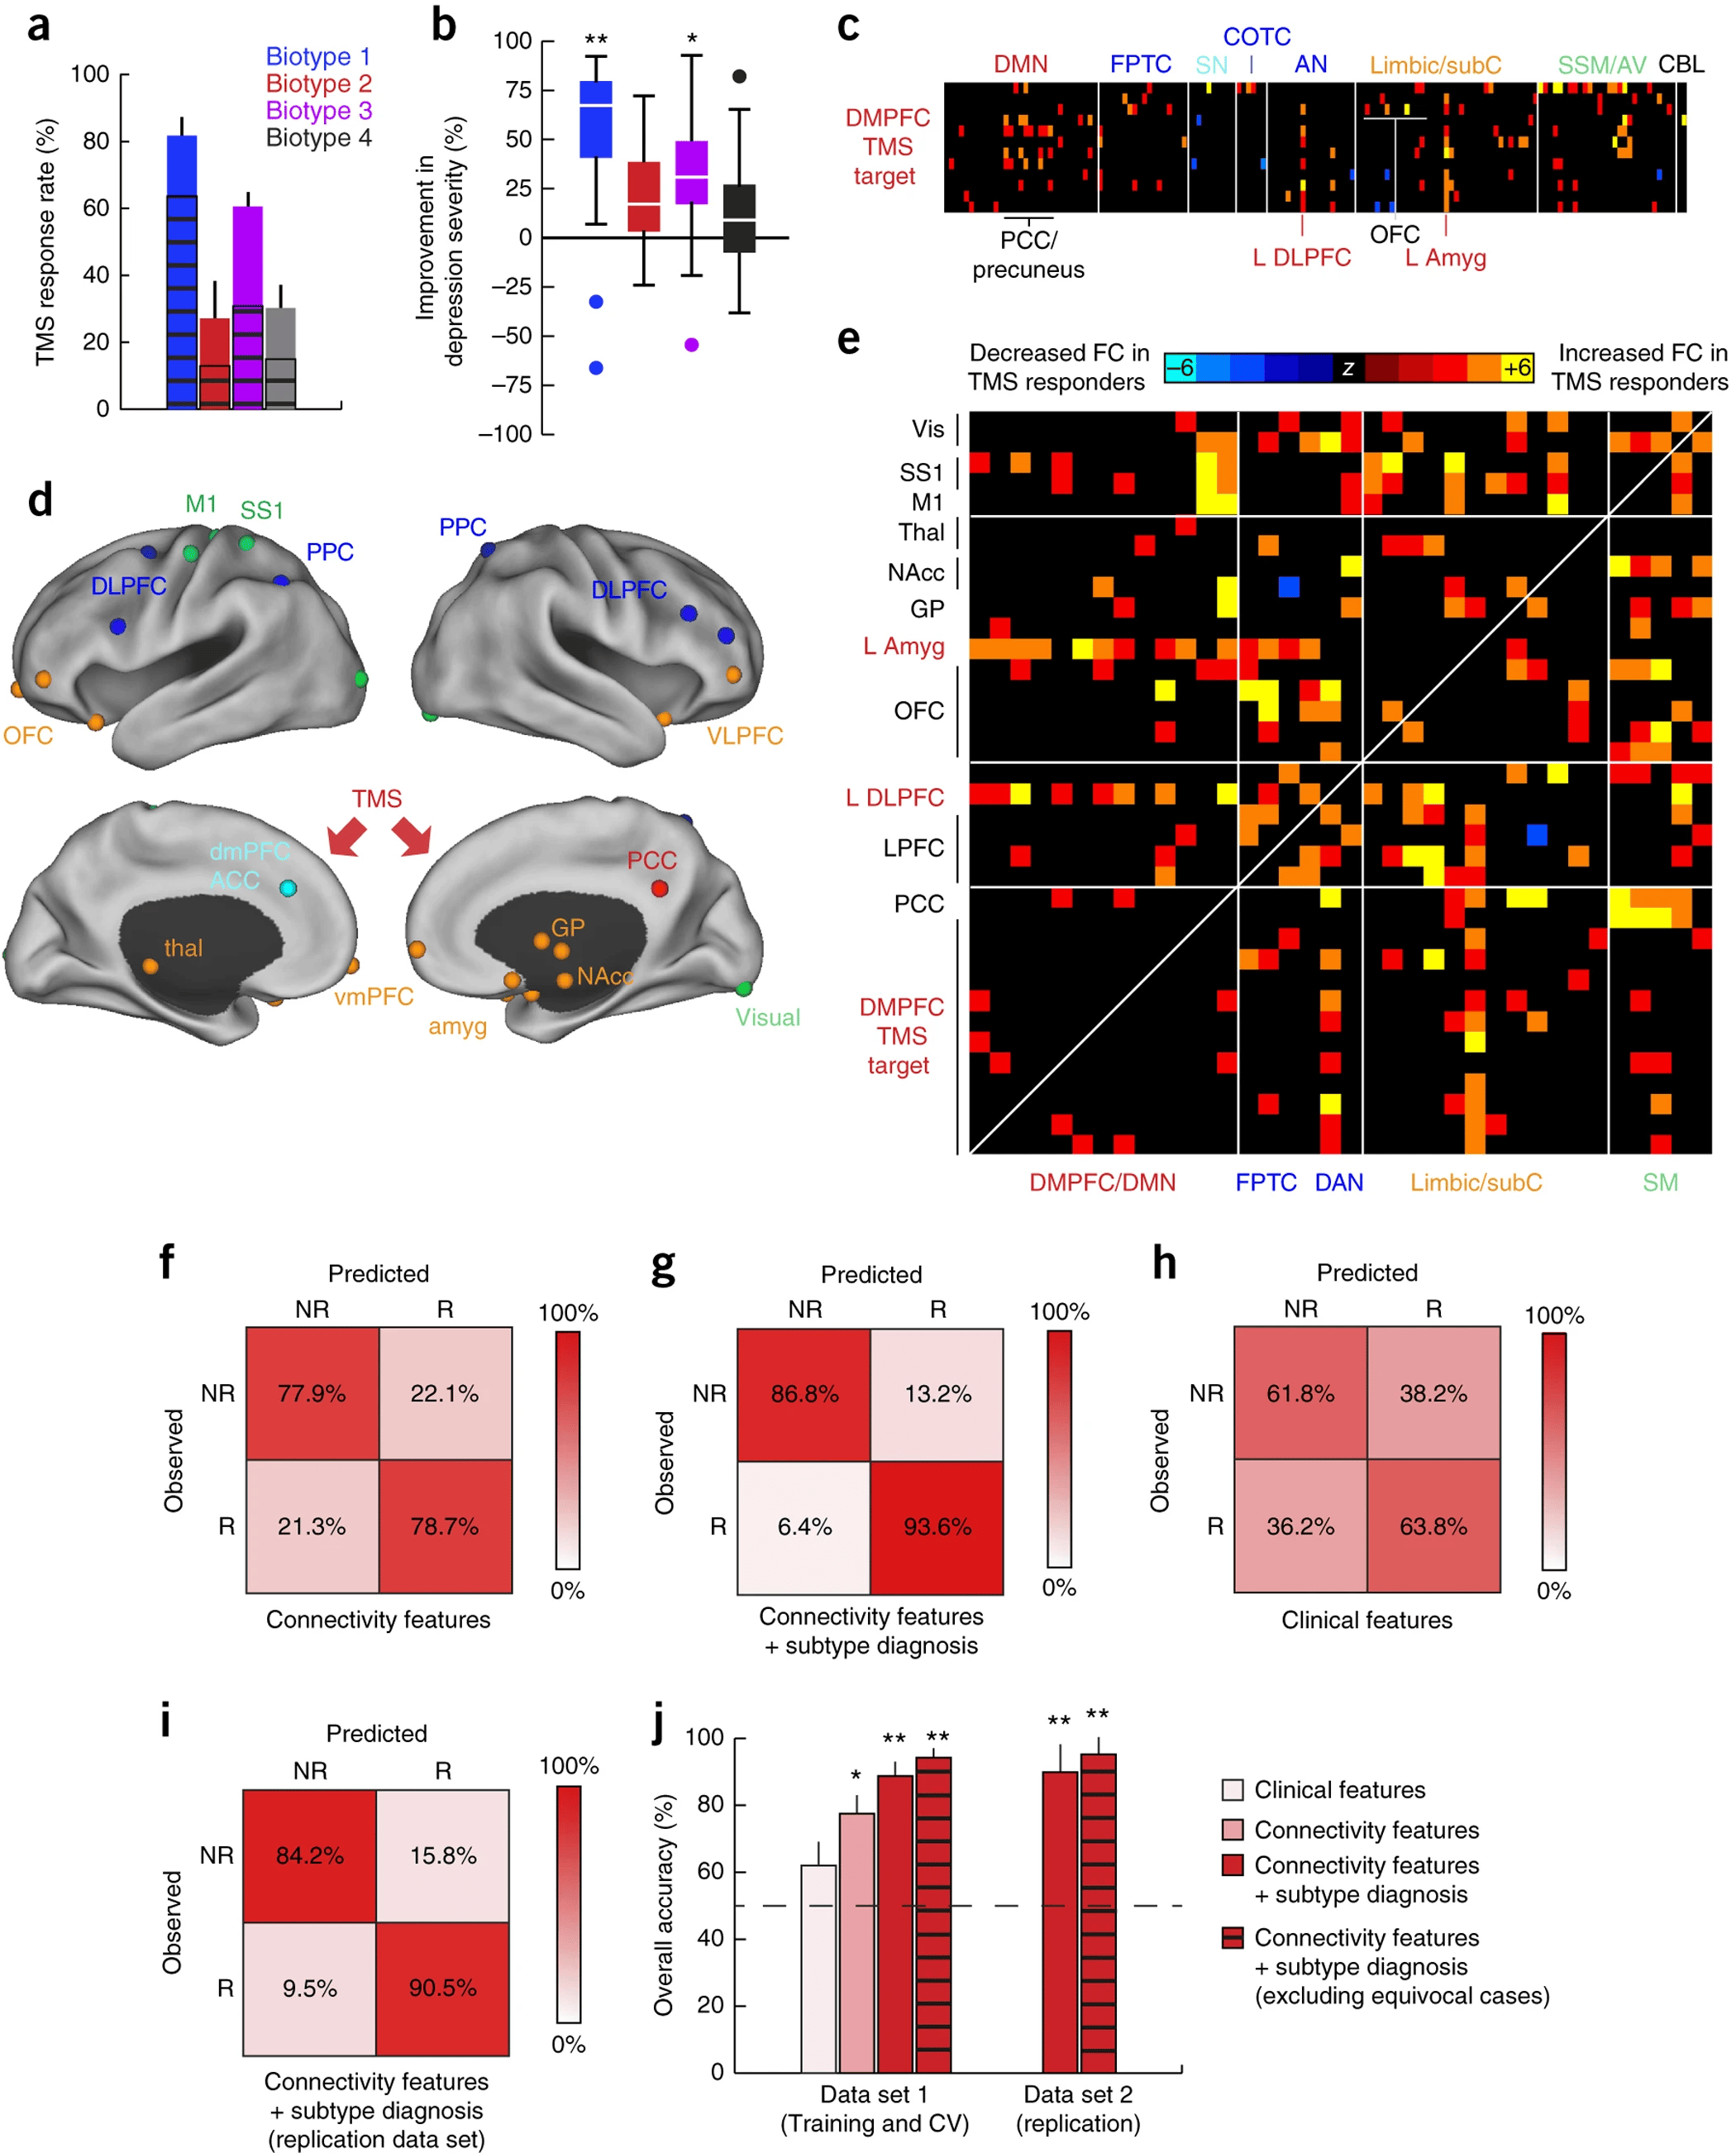
\includegraphics[height=7cm]{data/fig4.png}
            };
        }
        \visible<6>{
            \node[inner sep=0pt, draw=black] at (0, 0) {
                
\includegraphics[width=7cm]{data/dinga1.png}
            };
        }
        \visible<7>{
            \node[inner sep=0pt, draw=black] at (0, 0) {
                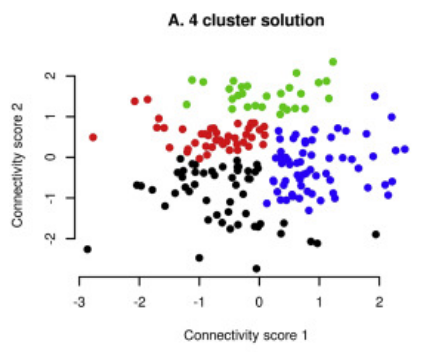
\includegraphics[width=5cm]{data/dinga2.png}
            };
        }
        \visible<8>{
            \node[inner sep=0pt, draw=black] at (0, 0) {
                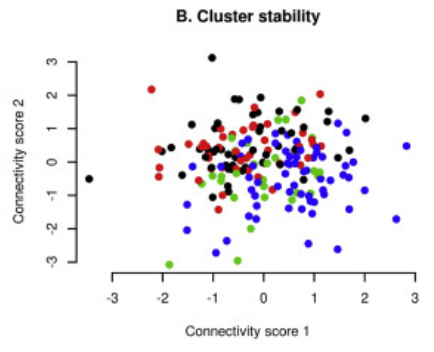
\includegraphics[width=5cm]{data/dinga3.png}
            };
        }
        \visible<9>{
            \node[text width=10.5cm] at (0, 0) {
                How can we avoid ending up in a clustering nightmare? \emoji{face-screaming-in-fear}
                \begin{itemize}
                    \item Quantitative evaluation of our clusters (see for instance Elements of Statistical Learning)
                    \item Test cluster stability via cross-validation, half-split tests, bootstrap etc.
                    \item Be cautious in interpretations
                \end{itemize}
            };
        }
    \end{tikzpicture}
\end{frame}


\end{document}
